\section{Collusion When Demand Fluctuates}\label{sec:12-demand}

The supergames of \cref{sec:12-perfect} hold demand fixed. Real markets move with the seasons, the business cycle
and shifts in tastes. This section asks how such movements change what a cartel can sustain. The answer rests on
one comparison. In each period a firm weighs the gain from undercutting today against the collusive profit it loses
in the punishment that follows. The gain depends on current demand. The loss depends on expected future demand.
When demand fluctuates, both sides of the incentive constraint move, and they need not move together.

The models of this section differ in how today's demand predicts future demand. If demand shocks are independent
over time and observed by the firms, the future loss is the same in every state, while the gain is largest when
demand is high. Collusion is then hardest in booms, and collusive margins are countercyclical
\citep{RotembergSaloner1986}. If demand follows a predictable cycle, the future loss is small when demand is about
to fall \citep{HaltiwangerHarrington1991}. If booms and recessions are persistent phases of growth, the future loss
is larger in the phase that predicts higher future demand \citep{BagwellStaiger1997}. In all three models firms
observe demand, so the most collusive equilibrium has no price war on its equilibrium path. Price wars on the path
appear when demand is unobserved, the case of \citet{GreenPorter1984} in \cref{sec:12-public}.

Throughout this section $\delta$ is the discount factor. The state of demand in period $t$ is $\omega_t$. The
papers write $\epsilon_t$ for it, a symbol the book reserves for taste shocks. Market demand in state $\omega$ is
$D(p,\omega)$, and industry profit at a common price $p$ is $\pi(p,\omega) = (p-c)D(p,\omega)$. The monopoly price is
$p^m(\omega)$ and monopoly profit is $\pi^m(\omega) = \pi(p^m(\omega),\omega)$. When we quote a paper's equations we
translate them into this notation.

\subsection{A two-state model}\label{sec:12-rs-two-state}

We begin with two demand states. This version shows the logic of \citet{RotembergSaloner1986} in a few lines and
produces four regimes of optimal collusion.

\begin{assumption}[Two independent demand states]\label{asm:12-two-state}
\leavevmode
\begin{enumerate}[label=(\roman*)]
\item $N \ge 2$ firms sell a homogeneous good at constant marginal cost $c$. In each period $t = 0, 1, 2, \dots$ they
set prices simultaneously. The firm with the lowest price serves the market, and firms tied at the lowest price
share it equally.
\item Market demand is $D_H(p)$ in the high state and $D_L(p)$ in the low state. Each state occurs with probability
$\frac{1}{2}$, independently across periods, and $D_H(p) > D_L(p)$ at every price.
\item All firms observe the state before they set prices, and all past prices are observed.
\item Industry profit $\pi_s(p) = (p-c)D_s(p)$ has a unique maximizer $p_s^M$ and is strictly increasing on
$[c, p_s^M]$. We write $\pi_s^M = \pi_s(p_s^M)$ for $s \in \{H, L\}$.
\item Firms maximize expected discounted profit with discount factor $\delta \in (0,1)$.
\end{enumerate}
\end{assumption}

Since $D_H > D_L$, we have $\pi_H(p) > \pi_L(p)$ at every $p > c$. Hence $\pi_H^M \ge \pi_H(p_L^M) > \pi_L^M$. In
this subsection $H$ and $L$ name states. They are not the Herfindahl index or a number of periods.

The firms consider the strategy profile
\begin{equation}\label{eq:12-two-state-strategy}
p_{it}(h^t) =
\begin{cases}
p_H & \text{if no firm has deviated before } t \text{ and the state is } H,\\
p_L & \text{if no firm has deviated before } t \text{ and the state is } L,\\
c & \text{if some firm has deviated before } t,
\end{cases}
\end{equation}
where $h^t$ records past prices and states. The third line is Bertrand reversion. It gives every firm zero profit,
which is the minmax payoff of the stage game (\cref{lem:12-ir}), so no credible punishment is harsher. We
restrict attention to prices $p_s \in [c, p_s^M]$. A price above $p_s^M$ is never useful. A deviator could then
charge $p_s^M$ and earn $\pi_s^M$. Replacing $p_s$ by the price below $p_s^M$ with the same profit leaves the future
unchanged and lowers the deviation payoff.

\casehead{The incentive constraints}
Let
\begin{equation}\label{eq:12-two-state-V}
V \equiv \frac{1}{2}\pi_H(p_H) + \frac{1}{2}\pi_L(p_L)
\end{equation}
be expected industry profit per period on the collusive path. Consider a period in state $s$ with no earlier
deviation. A firm that conforms earns $\frac{1}{N}\pi_s(p_s)$ today. From tomorrow on it earns $\frac{V}{N}$ per period in
expectation. Because states are independent over time, this expectation does not depend on today's state. The
discounted value of the future is
\begin{equation*}
\sum_{\tau = 1}^{\infty} \delta^{\tau}\frac{V}{N} = \frac{\delta}{1-\delta}\,\frac{V}{N}.
\end{equation*}
The best deviation undercuts to $p_s - \varepsilon'$ for a small $\varepsilon' > 0$. (We write $\varepsilon'$ for the price
cut because $\varepsilon$ is an elasticity.) The deviator serves the whole market and earns $\pi_s(p_s - \varepsilon')$,
which tends to $\pi_s(p_s)$ as $\varepsilon' \to 0$. Afterwards every firm prices at $c$, and the deviator earns zero.
Conforming is optimal if
\begin{equation*}
\pi_s(p_s) \le \frac{1}{N}\pi_s(p_s) + \frac{\delta}{1-\delta}\,\frac{V}{N}.
\end{equation*}
Subtracting $\frac{1}{N}\pi_s(p_s)$ from both sides gives
\begin{equation}\label{eq:12-two-state-ic}
\frac{N-1}{N}\,\pi_s(p_s) \le \frac{\delta}{1-\delta}\,\frac{1}{N}\left[\frac{1}{2}\pi_H(p_H) + \frac{1}{2}\pi_L(p_L)\right],
\qquad s \in \{H, L\}.
\end{equation}

\begin{proposition}[Incentive constraints with two demand states]\label{prop:12-rs-two-state-ic}
Under \cref{asm:12-two-state}, with $p_s \in [c, p_s^M]$ for $s = H, L$, the profile \eqref{eq:12-two-state-strategy}
is a subgame perfect equilibrium if and only if \eqref{eq:12-two-state-ic} holds in both states.
\end{proposition}

\begin{proof}
After a deviation the profile prescribes the static Nash equilibrium in every period, whatever happens. This is
subgame perfect by \cref{prop:12-static-repeat}. On the collusive path, the one-shot deviation principle
(\cref{prop:12-osdp}) lets us check single deviations. A price above $p_s$ sells nothing today and leads to zero
profit forever, so it is never better than conforming. A price $p' < p_s$ earns $\pi_s(p') < \pi_s(p_s)$ today, because
$\pi_s$ is strictly increasing on $[c, p_s^M]$, and zero afterwards. If \eqref{eq:12-two-state-ic} holds, every such
deviation pays strictly less than conforming. If \eqref{eq:12-two-state-ic} fails in state $s$, then
$\pi_s(p_s)$ exceeds the conforming payoff. By continuity, $\pi_s(p')$ also exceeds it for $p'$ close enough to
$p_s$, and that deviation is profitable.
\end{proof}

The left side of \eqref{eq:12-two-state-ic} is the current gain from cheating. It is larger in the high state,
because a deviator steals a larger market. The right side is the future loss from the price war. It is the same in
both states, because independent shocks make tomorrow's expected demand the same whatever happens today. The
temptation is therefore strongest in the high state.

\casehead{Optimal collusion}
Define the \emph{slack factor}
\begin{equation}\label{eq:12-kappa}
\kappa \equiv \frac{\delta}{(1-\delta)(N-1)}.
\end{equation}
It rises with $\delta$, falls with $N$, and equals one exactly when $\delta = \frac{N-1}{N}$, the patience threshold of
\cref{prop:12-bertrand}. Multiplying \eqref{eq:12-two-state-ic} by $\frac{N}{N-1}$ gives
\begin{equation}\label{eq:12-two-state-kappa}
\pi_s(p_s) \le \kappa V, \qquad s = H, L.
\end{equation}
\emph{Optimal collusion} selects the most collusive equilibrium in the sense of \cref{sec:12-folk}: the subgame
perfect equilibrium that maximizes the firms' expected profit $V$. It is
convenient to choose profit levels $v_s = \pi_s(p_s) \in [0, \pi_s^M]$ instead of prices. Because $\pi_s$ is strictly
increasing on $[c, p_s^M]$, each $v_s$ determines $p_s$ uniquely. Substituting $V = \frac{1}{2}(v_H + v_L)$ into
\eqref{eq:12-two-state-kappa} and collecting terms gives
\begin{equation*}
\left(1 - \frac{\kappa}{2}\right) v_H \le \frac{\kappa}{2}\, v_L, \qquad \left(1 - \frac{\kappa}{2}\right) v_L \le \frac{\kappa}{2}\, v_H .
\end{equation*}
If $\kappa \ge 2$ both constraints hold for all profit levels. If $\kappa < 2$ they read $v_H \le r v_L$ and
$v_L \le r v_H$ with $r \equiv \frac{\kappa}{2 - \kappa}$. Problems of this form recur in this section, so we solve them once.

\begin{lemma}[Greatest point of a pair of linked constraints]\label{lem:12-two-constraint}
Let $X_1, X_2 > 0$ and $a_1, a_2 \in (0, +\infty]$, where $a_i = +\infty$ means that the corresponding constraint is
absent. Let
\begin{equation*}
S = \left\{ (x_1, x_2) \in [0, X_1] \times [0, X_2] : x_1 \le a_1 x_2,\ x_2 \le a_2 x_1 \right\}.
\end{equation*}
\begin{enumerate}[label=(\roman*)]
\item If $a_1 a_2 < 1$, then $S = \{(0,0)\}$.
\item If $a_1 a_2 \ge 1$, then $x^* = \left(\min\{X_1, a_1 X_2\},\ \min\{X_2, a_2 X_1\}\right)$ belongs to $S$ and
$x^* \ge x$ componentwise for every $x \in S$. At most one coordinate of $x^*$ lies below its cap $X_i$.
\end{enumerate}
\end{lemma}

\begin{proof}
(i) If $a_1 a_2 < 1$, both $a_i$ are finite. For $x \in S$, $x_1 \le a_1 x_2 \le a_1 a_2 x_1$, so
$(1 - a_1a_2)x_1 \le 0$ and $x_1 = 0$. Then $x_2 \le a_2 x_1 = 0$.

(ii) Every $x \in S$ satisfies $x_1 \le \min\{X_1, a_1 x_2\} \le \min\{X_1, a_1 X_2\} = x_1^*$, and likewise
$x_2 \le x_2^*$. It remains to show $x^* \in S$. Suppose first that both coordinates are capped, $x^* = (X_1, X_2)$.
Then $X_1 \le a_1 X_2$ and $X_2 \le a_2 X_1$, so $x^* \in S$. Suppose next that $a_2 X_1 < X_2$, so
$x^* = (\min\{X_1, a_1X_2\}, a_2 X_1)$. Since $a_1 X_2 > a_1 a_2 X_1 \ge X_1$, the first coordinate equals $X_1$. The
constraints read $X_1 \le a_1 a_2 X_1$, which holds, and $a_2 X_1 \le a_2 X_1$. The case $a_1 X_2 < X_1$ is symmetric.
Both coordinates cannot fall below their caps, because $a_1 X_2 < X_1$ and $a_2 X_1 < X_2$ together imply
$a_1 a_2 < 1$.
\end{proof}

The greatest point maximizes every coordinate at once. It therefore maximizes any objective that increases in both
coordinates, such as the cartel's expected profit.

\begin{proposition}[Four regimes of optimal collusion]\label{prop:12-rs-regimes}
Let \cref{asm:12-two-state} hold and define
\begin{equation}\label{eq:12-kappa-bar}
\bar\kappa \equiv \frac{2\pi_H^M}{\pi_H^M + \pi_L^M} \in (1, 2), \qquad
\bar\delta \equiv \frac{\bar\kappa (N-1)}{1 + \bar\kappa(N-1)}.
\end{equation}
The most collusive equilibrium of the form \eqref{eq:12-two-state-strategy} is as follows.
\begin{enumerate}[label=(\roman*)]
\item \emph{Regime 1} ($\kappa \ge \bar\kappa$, equivalently $\delta \ge \bar\delta$). Firms charge the monopoly price
in both states.
\item \emph{Regime 2} ($1 < \kappa < \bar\kappa$). Firms charge $p_L = p_L^M$. The boom price $p_H < p_H^M$ is the
price on the increasing branch of $\pi_H$ that solves
\begin{equation}\label{eq:12-two-state-regime2}
\pi_H(p_H) = \frac{\kappa\,\pi_L^M}{2 - \kappa}.
\end{equation}
\item \emph{Regime 3} ($\kappa = 1$, equivalently $\delta = \frac{N-1}{N}$). Both constraints bind,
$\pi_H(p_H) = \pi_L(p_L) = \pi_L^M$, so $p_L = p_L^M$ and $p_H < p_L$.
\item \emph{Regime 4} ($\kappa < 1$). Only the competitive outcome $p_H = p_L = c$ is sustainable.
\end{enumerate}
\end{proposition}

\begin{proof}
Apply \cref{lem:12-two-constraint} with $x_1 = v_H$, $x_2 = v_L$, $X_1 = \pi_H^M$ and $X_2 = \pi_L^M$. If
$\kappa \ge 2$, set $a_1 = a_2 = +\infty$, and the greatest point is monopoly in both states. Since $\bar\kappa < 2$,
this case belongs to regime 1. If $\kappa < 2$, set $a_1 = a_2 = r = \frac{\kappa}{2-\kappa}$. Then $r < 1$ exactly
when $\kappa < 1$, and part (i) of the lemma gives regime 4. If $1 \le \kappa < 2$, then $r \ge 1$ and part (ii) gives
\begin{equation*}
v_L^* = \min\{\pi_L^M, r\pi_H^M\} = \pi_L^M, \qquad v_H^* = \min\{\pi_H^M, r\pi_L^M\},
\end{equation*}
where the first equality uses $r\pi_H^M \ge \pi_H^M > \pi_L^M$. The boom profit is capped below $\pi_H^M$ exactly
when $r\pi_L^M < \pi_H^M$. Substituting $r$ and rearranging,
\begin{equation*}
\kappa\,\pi_L^M < (2-\kappa)\,\pi_H^M \iff \kappa\left(\pi_H^M + \pi_L^M\right) < 2\pi_H^M \iff \kappa < \bar\kappa .
\end{equation*}
This yields regimes 1 and 2, with $v_H^* = r\pi_L^M$ in regime 2, which is \eqref{eq:12-two-state-regime2}. At
$\kappa = 1$ we have $r = 1$ and $v_H^* = v_L^* = \pi_L^M$. Then $\pi_H(p_H) = \pi_L(p_L^M) < \pi_H(p_L^M)$. If
$p_L^M \le p_H^M$, monotonicity of $\pi_H$ on $[c, p_H^M]$ gives $p_H < p_L^M$. If $p_L^M > p_H^M$, then
$p_H \le p_H^M < p_L^M$. Either way $p_H < p_L$. Finally, $\kappa \ge \bar\kappa$ means
$\frac{\delta}{1-\delta} \ge \bar\kappa(N-1)$, which rearranges to $\delta \ge \bar\delta$. The greatest point maximizes
$V$, so it is the most collusive equilibrium.
\end{proof}

Two checks are useful. Without fluctuations, $\pi_H^M = \pi_L^M$, so $\bar\kappa = 1$ and $\bar\delta = \frac{N-1}{N}$,
the threshold of the constant-demand Bertrand supergame. With fluctuations, $\bar\kappa - 1 =
\frac{\pi_H^M - \pi_L^M}{\pi_H^M + \pi_L^M}$. The range of discount factors with state-dependent pricing widens with the
dispersion of monopoly profits. The next result says when the boom price lies below the recession price.

\begin{corollary}[Countercyclical prices in regime 2]\label{cor:12-rs-countercyclical}
Suppose $p_L^M \le p_H^M$, so the monopoly price is weakly higher in the high state. In regime 2, $p_H < p_L$ if and
only if $\frac{\kappa}{2-\kappa} < \frac{\pi_H(p_L^M)}{\pi_L^M}$. The right side exceeds one, so the boom price is below the
recession price for all $\kappa$ in an interval above one. If instead $p_L^M > p_H^M$, then $p_H < p_L$ throughout
regimes 2 and 3.
\end{corollary}

\begin{proof}
In regime 2, $p_L = p_L^M$, and both $p_H$ and $p_L^M$ lie in $[c, p_H^M]$, where $\pi_H$ is strictly increasing. So
$p_H < p_L^M$ if and only if $\pi_H(p_H) < \pi_H(p_L^M)$. By \eqref{eq:12-two-state-regime2} this is
$\frac{\kappa}{2-\kappa}\pi_L^M < \pi_H(p_L^M)$. If $p_L^M > p_H^M$, then $p_H \le p_H^M < p_L^M = p_L$.
\end{proof}

\begin{example}[Multiplicative demand shocks]\label{ex:12-rs-multiplicative}
Let $D_s(p) = A_s(1-p)$ with $A_H > A_L > 0$ and $c = 0$. Then $\pi_s(p) = A_s p(1-p)$, so $p_H^M = p_L^M = \frac{1}{2}$ and
$\pi_s^M = \frac{A_s}{4}$. The threshold for full monopoly is $\bar\kappa = \frac{2A_H}{A_H + A_L}$. In regime 2,
\eqref{eq:12-two-state-regime2} becomes
\begin{equation*}
A_H\, p_H(1 - p_H) = \frac{\kappa A_L}{4(2-\kappa)} .
\end{equation*}
The lower root of this quadratic is
\begin{equation}\label{eq:12-two-state-example}
p_H = \frac{1}{2}\left[1 - \sqrt{1 - \frac{\kappa A_L}{(2-\kappa)A_H}}\right] < \frac{1}{2} = p_L .
\end{equation}
The recession price is the monopoly price, and the boom price is strictly lower throughout regime 2. Since $c = 0$,
the price is also the margin $p - c$, so margins are countercyclical. With $N = 2$, $A_H = 1.5$ and $A_L = 1$ we get
$\bar\kappa = 1.2$ and $\bar\delta = \frac{6}{11} \approx 0.545$. At $\kappa = 1$ the boom price is
$\frac{1}{2}\left(1 - \sqrt{1 - \frac{A_L}{A_H}}\right) \approx 0.211$. At $\delta = 0.52$, where $\kappa \approx 1.083$, it is
$p_H \approx 0.270$. \Cref{fig:12-rs-two-state} plots both prices against $\delta$.
\end{example}

\begin{figure}[htbp]
\centering
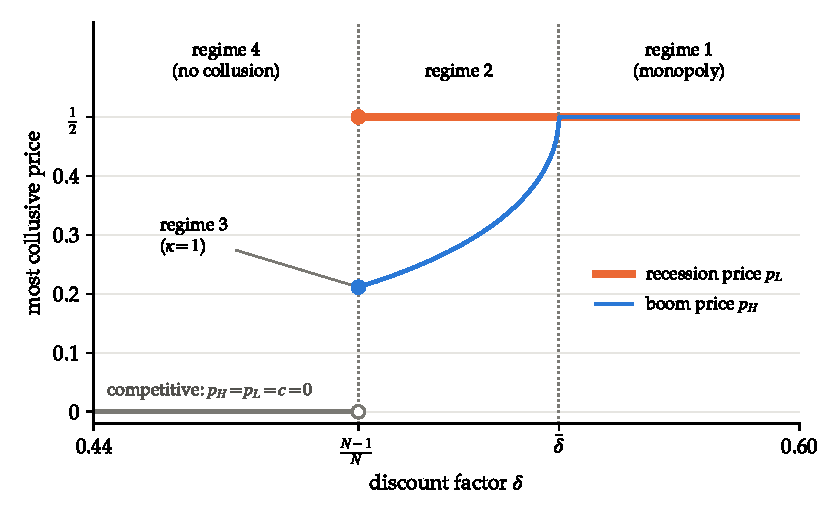
\includegraphics[width=0.78\textwidth]{figures/ch12/rs_two_state.pdf}
\caption{Most collusive prices in the two-state model of \cref{ex:12-rs-multiplicative}: $N = 2$, $c = 0$,
$D_s(p) = A_s(1-p)$ with $A_H = 1.5$ and $A_L = 1$, each state with probability $\frac{1}{2}$. Below
$\delta = \frac{N-1}{N} = \frac{1}{2}$ only competitive pricing is sustainable (regime 4). At $\delta = \frac{1}{2}$ both
constraints bind (regime 3). Between $\frac{1}{2}$ and $\bar\delta = \frac{6}{11}$ the recession price is the monopoly price
$\frac{1}{2}$ and the boom price is lower (regime 2). Above $\bar\delta$ both prices equal $\frac{1}{2}$ (regime 1). Script
\texttt{rs\_two\_state.py}.}
\label{fig:12-rs-two-state}
\end{figure}

\casehead{What the regimes mean}
In regime 2 the cartel concedes in the boom. It lowers the boom price until the gain from undercutting no longer
exceeds the future loss. It keeps the recession price at the monopoly level, because a higher recession profit
raises $V$ and relaxes the boom constraint as well. The result is a pricing pattern that \citet{RotembergSaloner1986}
call a \emph{price war during a boom}: a period of low prices and margins when demand is high. Nobody cheats. The low
boom price is part of the collusive agreement, chosen so that nobody wants to cheat.

Three caveats follow from the proposition. The prediction of countercyclical margins needs optimal collusion. The
competitive outcome is also an equilibrium for every $\delta$, and so is constant pricing at any price that satisfies
both constraints. The prediction also needs intermediate patience. In the example, cyclical pricing occurs only for
$\delta \in [0.5, 0.545)$. Finally, it relies on independent shocks. With persistent demand the future loss depends on
today's state, and the conclusion can reverse, as \cref{sec:12-hh,sec:12-bs} show. Regime 3 is a knife-edge case
with two states. With a continuum of states, profits are capped at a common level in all high states, and this
pattern holds for an interval of discount factors. We turn to that model now.

\subsection{Rotemberg and Saloner (1986): price wars during booms}\label{sec:12-rs}

\subsubsection{The question}

\citet{RotembergSaloner1986} ask how implicitly colluding oligopolists behave when demand fluctuates. Their paper has
two objectives (p.~1). The first is to describe oligopoly pricing over the business cycle. The second is to ask
whether this pricing itself causes business cycles and sticky prices. Their basic point is that collusion is harder
when demand is high. In a boom, ``chiseling away from the collusive level of output becomes more profitable for each
individual firm'' (p.~1), so the oligopoly can sustain only a less collusive outcome. An oligopoly that becomes more
competitive in booms expands output. If its output is an input to other
sectors, their output can rise too. This produces the comovement of outputs that characterizes business cycles.

The question matters for industrial organization because it overturns a piece of folklore. \citet{Scherer1980}
wrote that price cutting ``runs most rampant among oligopolists with high fixed costs'' precisely when business
conditions turn sour (his p.~208, quoted on p.~24). Rotemberg and Saloner concede that one can build models in which recessions
cause price wars. ``Our basis for rejecting this folklore is not theoretical,'' they write. ``Instead our rejection is
based on facts'' (p.~4). We work from the 1984 working paper \citep{RotembergSaloner1984}, which contains the model,
the macroeconomic application and the evidence. Page and table numbers in this subsection refer to it.

\needspace{8\baselineskip}
\subsubsection{The model}

\begin{assumption}[Observable independent demand shocks]\label{asm:12-rs}
\leavevmode
\begin{enumerate}[label=(\roman*)]
\item $N \ge 2$ symmetric firms sell a homogeneous good at constant marginal cost $c$ and set prices simultaneously in
each period. The lowest price serves the market, and ties split it equally.
\item Demand in period $t$ is $D(p, \omega_t)$. The state $\omega_t$ is independent and identically distributed over
time, with CDF $F_\omega$ whose support is $[\underline\omega, \bar\omega]$.
\item All firms learn $\omega_t$ before they set prices, and all past prices are observed.
\item For each $\omega$, $\pi(p,\omega)$ is continuous, strictly increasing in $p$ on $[c, p^m(\omega)]$, and uniquely
maximized at $p^m(\omega)$, with $\pi^m(\omega) > 0$.
\item For each $p > c$, $\pi(p,\omega)$ is strictly increasing in $\omega$. The function $\pi^m$ is continuous and
$\E[\pi^m(\omega)] < \infty$.
\item Firms discount the future with factor $\delta \in (0,1)$.
\end{enumerate}
\end{assumption}

Part (v) says that a higher state shifts demand out. It implies that monopoly profit rises with the state, since for
$\omega' > \omega$ we have $\pi^m(\omega') \ge \pi(p^m(\omega), \omega') > \pi^m(\omega)$. The timing in (iii) is the
model's defining feature. Punishments depend on future states, so their expected size depends on the distribution of
$\omega$. The reward from cheating depends on the current state, which firms see. The authors show that ``for a wide
variety of interesting cases the reward for cheating from the joint profit-maximizing level is monotonically
increasing in $\epsilon_t$'' (pp.~6--7). Here $\epsilon_t$ is the paper's symbol for $\omega_t$.

A \emph{collusive scheme} is a price schedule $p(\cdot)$ that assigns a price to each state. On the collusive path,
every firm charges $p(\omega_t)$. After any deviation, all firms charge $c$ forever. This Nash reversion holds every
firm to its minmax payoff of zero, so it is the harshest credible punishment. Any outcome that some subgame perfect
equilibrium sustains can therefore be sustained with Nash reversion. The authors make the same point about infinite
reversion. ``This length is optimal since it is the biggest credible threat and since, along the equilibrium path,
firms never find themselves punishing each other'' (p.~2). They also note that infinite punishments are less compelling if
industry membership changes, and they use low discount factors in their numerical examples for that reason (p.~8).

As in \cref{sec:12-rs-two-state}, we may restrict attention to $p(\omega) \in [c, p^m(\omega)]$. Write
$v(\omega) = \pi(p(\omega), \omega)$ for industry profit in state $\omega$ on the collusive path, and
$\bar E = \E[v(\omega)]$ for its expectation. The argument that led to \eqref{eq:12-two-state-ic} applies state by
state. A firm that conforms in state $\omega$ earns $\frac{1}{N}v(\omega) + \frac{\delta}{1-\delta}\frac{\bar E}{N}$, and the best
deviation earns $v(\omega)$. The incentive constraint is
\begin{equation*}
\frac{N-1}{N}\, v(\omega) \le \frac{\delta}{1-\delta}\,\frac{\bar E}{N} \qquad \text{for all } \omega.
\end{equation*}
With the slack factor $\kappa$ of \eqref{eq:12-kappa} it reads
\begin{equation}\label{eq:12-rs-ic}
v(\omega) \le \kappa\, \bar E \qquad \text{for all } \omega \in [\underline\omega, \bar\omega].
\end{equation}
The cap $\kappa \bar E$ is the same in every state, because the future does not depend on the present. The cap is
also endogenous. A scheme that earns more on average can afford higher profit in each state.

The paper writes the same condition in terms of the \emph{punishment}
$K = \frac{\delta}{1-\delta}\E[\text{per-firm profit}]$, the expected discounted profit a deviator forfeits (eq.~(1), p.~8).
This $K$ is the paper's symbol and has nothing to do with the capacity of \cref{ex:12-capacity}. A
firm deviates from joint profit maximization in state $\epsilon_t$ if $(N-1)\Pi^m > K$, where $\Pi^m$ is per-firm
monopoly profit (p.~7). The sustainable per-firm profit in high states is $\frac{K}{N-1}$ (eq.~(2), p.~9). In our
notation $K = \frac{\delta \bar E}{(1-\delta)N}$, so the per-firm cap $\frac{K}{N-1}$ equals $\frac{\kappa\bar E}{N}$, which is
\eqref{eq:12-rs-ic} divided by $N$.

\subsubsection{The most collusive scheme as a fixed point}

Every sustainable scheme satisfies $v(\omega) \le \min\{\pi^m(\omega), \kappa\bar E\}$. This suggests the map
\begin{equation}\label{eq:12-rs-h}
h(E) \equiv \E_\omega\left[\min\left\{\pi^m(\omega),\ \kappa E\right\}\right], \qquad E \ge 0,
\end{equation}
which gives the expected profit of the scheme that charges monopoly prices wherever the cap $\kappa E$ allows it.
The map $h$ is continuous and nondecreasing, $h(0) = 0$, and $h(E) \le \E[\pi^m] < \infty$. It is also concave, as
the expectation of a minimum of two functions that are linear in $E$.

\begin{lemma}[Sustainable profit levels]\label{lem:12-rs-fixed}
Under \cref{asm:12-rs}:
\begin{enumerate}[label=(\alph*)]
\item A number $E \ge 0$ is the expected profit of some sustainable scheme if and only if $E \le h(E)$.
\item Let $E^*$ be the largest $E$ with $E \le h(E)$. Then $E^* = h(E^*)$, so $E^*$ is the largest fixed point of $h$.
\item The scheme $v^*(\omega) = \min\{\pi^m(\omega), \kappa E^*\}$ is sustainable. Every sustainable scheme satisfies
$v(\omega) \le v^*(\omega)$ in every state.
\end{enumerate}
\end{lemma}

\begin{proof}
(a) If $v$ is sustainable with mean $E$, then $v(\omega) \le \min\{\pi^m(\omega), \kappa E\}$ for all $\omega$. Taking
expectations, $E \le h(E)$. Conversely, $E = 0$ is the mean of the competitive scheme. If $0 < E \le h(E)$, define
\begin{equation*}
v(\omega) = \frac{E}{h(E)}\min\left\{\pi^m(\omega), \kappa E\right\}.
\end{equation*}
Its mean is $E$. Since $\frac{E}{h(E)} \le 1$, it satisfies $v(\omega) \le \pi^m(\omega)$ and $v(\omega) \le \kappa E$ in every
state. The second inequality is \eqref{eq:12-rs-ic} at mean $E$, so $v$ is sustainable.

(b) The set $\{E \ge 0 : E \le h(E)\}$ is closed, by continuity, and bounded by $\E[\pi^m]$. So it has a largest element
$E^*$. Suppose $E^* < h(E^*)$. Let $E' = h(E^*)$. Since $h$ is nondecreasing, $h(E') \ge h(E^*) = E'$, so $E'$ belongs
to the set and exceeds $E^*$, a contradiction.

(c) Sustainability of $v^*$ follows from (a) and $E^* = h(E^*)$. If $v$ is sustainable with mean $\bar E$, then
$\bar E \le E^*$ by (a) and (b), so $v(\omega) \le \min\{\pi^m(\omega), \kappa\bar E\} \le v^*(\omega)$.
\end{proof}

Part (c) says that the most collusive scheme is the best for the firms in every state at once. There is no tradeoff
between states, so ``most collusive'' is well defined. The paper describes the same construction as a mapping from
punishments to cutoffs and back to punishments, and selects the greatest fixed point (pp.~9--10).

\begin{proposition}[Collusion with observable independent shocks]\label{prop:12-rs-threshold}
Let \cref{asm:12-rs} hold and let $E^*$ be the largest fixed point of $h$.
\begin{enumerate}[label=(\roman*)]
\item If $\kappa < 1$, equivalently $\delta < \frac{N-1}{N}$, then $E^* = 0$. Only competitive pricing is sustainable.
\item If $\kappa = 1$, then $E^* = \pi^m(\underline\omega)$. Industry profit is the same in every state, equal to the
monopoly profit of the lowest state.
\item If $\kappa > 1$, then $E^* > 0$ and $\kappa E^* > \pi^m(\underline\omega)$. Firms charge monopoly prices in every
state if and only if $\kappa\,\E[\pi^m(\omega)] \ge \pi^m(\bar\omega)$. Otherwise there is a cutoff
$\omega^* \in (\underline\omega, \bar\omega)$ with $\pi^m(\omega^*) = \kappa E^*$, and
\begin{equation}\label{eq:12-rs-schedule}
v^*(\omega) =
\begin{cases}
\pi^m(\omega) & \text{if } \omega \le \omega^*,\\
\kappa E^* = \pi^m(\omega^*) & \text{if } \omega > \omega^* .
\end{cases}
\end{equation}
The cutoff solves
\begin{equation}\label{eq:12-rs-cutoff}
\pi^m(\omega^*)\left[1 - \kappa\left(1 - F_\omega(\omega^*)\right)\right] = \kappa \int_{\underline\omega}^{\omega^*} \pi^m(\omega)\, \dd F_\omega(\omega).
\end{equation}
\item The values $E^*$ and $\kappa E^*$ and the cutoff $\omega^*$ are nondecreasing in $\kappa$. They are therefore
nondecreasing in $\delta$ and nonincreasing in $N$.
\end{enumerate}
\end{proposition}

\begin{proof}
(i) If $\kappa < 1$ and $E > 0$, then $h(E) \le \kappa E < E$. So the only fixed point is $E^* = 0$.

(ii) If $\kappa = 1$, then $h(E) = \E[\min\{\pi^m(\omega), E\}] \le E$, with equality if and only if $\pi^m(\omega) \ge E$
with probability one. Because $\underline\omega$ is in the support and $\pi^m$ is continuous and increasing, this
holds if and only if $E \le \pi^m(\underline\omega)$. The fixed points form the interval $[0, \pi^m(\underline\omega)]$,
and the largest is $\pi^m(\underline\omega)$. Then $v^*(\omega) = \min\{\pi^m(\omega), \pi^m(\underline\omega)\} =
\pi^m(\underline\omega)$ in every state.

(iii) Let $\phi(E) = h(E) - E$. For $0 < E \le \frac{\pi^m(\underline\omega)}{\kappa}$, the cap $\kappa E$ lies below
$\pi^m(\omega)$ in every state, so $h(E) = \kappa E$ and $\phi(E) = (\kappa - 1)E > 0$. As $E \to \infty$,
$\phi(E) \le \E[\pi^m] - E \to -\infty$. By continuity $\phi$ has a root above $\frac{\pi^m(\underline\omega)}{\kappa}$,
so $E^* > \frac{\pi^m(\underline\omega)}{\kappa} > 0$.

If $\kappa\E[\pi^m] \ge \pi^m(\bar\omega)$, then $h(\E[\pi^m]) = \E[\pi^m]$, because the cap never binds. No
fixed point exceeds $\E[\pi^m]$, so $E^* = \E[\pi^m]$ and $v^* = \pi^m$. Conversely, if $v^* = \pi^m$ almost surely,
then $E^* = \E[\pi^m]$ and $\pi^m(\omega) \le \kappa\E[\pi^m]$ for almost every $\omega$, hence at $\bar\omega$ by
continuity.

Otherwise $\pi^m(\underline\omega) < \kappa E^* < \pi^m(\bar\omega)$. Since $\pi^m$ is continuous and strictly
increasing, there is a unique $\omega^*$ with $\pi^m(\omega^*) = \kappa E^*$, and $v^*$ takes the form
\eqref{eq:12-rs-schedule}. The fixed-point condition $E^* = h(E^*)$ reads
\begin{equation*}
E^* = \int_{\underline\omega}^{\omega^*} \pi^m(\omega)\, \dd F_\omega(\omega) + \left(1 - F_\omega(\omega^*)\right)\kappa E^* .
\end{equation*}
Substitute $E^* = \frac{\pi^m(\omega^*)}{\kappa}$ and multiply by $\kappa$:
\begin{equation*}
\pi^m(\omega^*) = \kappa\int_{\underline\omega}^{\omega^*} \pi^m(\omega)\, \dd F_\omega(\omega) + \kappa\left(1 - F_\omega(\omega^*)\right)\pi^m(\omega^*).
\end{equation*}
Collecting the terms in $\pi^m(\omega^*)$ gives \eqref{eq:12-rs-cutoff}.

(iv) Write $h_\kappa$ to show the dependence on $\kappa$. For $\kappa' > \kappa$, $h_{\kappa'}(E) \ge h_\kappa(E)$ for all $E$.
So $E^*_\kappa = h_\kappa(E^*_\kappa) \le h_{\kappa'}(E^*_\kappa)$. By \cref{lem:12-rs-fixed}(a) and (b), $E^*_{\kappa'} \ge E^*_\kappa$.
Then $\kappa' E^*_{\kappa'} \ge \kappa E^*_\kappa$, and the cutoff $\omega^* = (\pi^m)^{-1}(\kappa E^*)$ rises weakly. Finally,
$\kappa$ increases in $\delta$ and decreases in $N$.
\end{proof}

Part (i) says that demand fluctuations do not change the patience needed for any collusion at all. Some collusion is
possible exactly when $\delta \ge \frac{N-1}{N}$, as with constant demand. Fluctuations change the form of collusion
above that threshold. Part (iv) restates two claims of the paper (p.~11). The set of states with monopoly pricing
shrinks as $N$ grows, ``as in Stigler's model'' \citep{Stigler1964}. It also shrinks as the future becomes less
important.

\begin{remark}[The existence conditions in the working paper]\label{rem:12-rs-wp}
The working paper states two sufficient conditions for an interior cutoff (pp.~9--10). Its condition (ii) says that
monopoly profit in the highest state exceeds $\kappa$ times its mean, which is the failure of full monopoly in
\cref{prop:12-rs-threshold}(iii). Its condition (i), which should ensure that some collusion is possible, is stated in
a form that appears to come from typographical sign errors in its equations (3) and (5). We have derived the
conditions directly. Collusion is possible if and only if $\kappa \ge 1$, and an interior cutoff exists if and only if
in addition $\kappa\,\E[\pi^m] < \pi^m(\bar\omega)$.
\end{remark}

\subsubsection{The price schedule}

The profit schedule \eqref{eq:12-rs-schedule} translates into prices. Below the cutoff the cartel charges the monopoly
price. Above it, profit must stay at the cap $\kappa E^*$ while demand keeps rising.

\begin{proposition}[Collusive prices fall in booms]\label{prop:12-rs-prices}
Let \cref{asm:12-rs} hold with $\kappa > 1$ and an interior cutoff $\omega^*$. Suppose $\pi$ is continuously
differentiable, $\pi_p > 0$ on $(c, p^m(\omega))$, and $\pi_\omega > 0$ for $p > c$. Let $p^*(\omega)$ be the most
collusive price schedule.
\begin{enumerate}[label=(\roman*)]
\item For $\omega \le \omega^*$, $p^*(\omega) = p^m(\omega)$.
\item For $\omega > \omega^*$, $p^*(\omega)$ is the unique $p \in (c, p^m(\omega))$ with $\pi(p, \omega) = \kappa E^*$, and
\begin{equation}\label{eq:12-rs-dpdw}
\frac{\dd p^*}{\dd \omega} = -\frac{\pi_\omega(p^*, \omega)}{\pi_p(p^*, \omega)} < 0 .
\end{equation}
\item For $\omega > \omega^*$, industry output $D(p^*(\omega), \omega)$ increases in $\omega$.
\item If $p^m$ is nondecreasing, then $p^*$ attains its maximum at $\omega^*$, and the ratio $\frac{p^*(\omega)}{p^m(\omega)}$
decreases strictly on $(\omega^*, \bar\omega]$.
\end{enumerate}
\end{proposition}

\begin{proof}
(i) is \eqref{eq:12-rs-schedule}. For (ii), fix $\omega > \omega^*$. Then $\pi(c, \omega) = 0 < \kappa E^* <
\pi^m(\omega)$. Since $\pi(\cdot, \omega)$ is continuous and strictly increasing on $[c, p^m(\omega)]$, there is exactly
one $p \in (c, p^m(\omega))$ with $\pi(p, \omega) = \kappa E^*$. Differentiate the identity $\pi(p^*(\omega), \omega) =
\kappa E^*$ with respect to $\omega$:
\begin{equation*}
\pi_p(p^*, \omega)\,\frac{\dd p^*}{\dd \omega} + \pi_\omega(p^*, \omega) = 0 .
\end{equation*}
Solving gives \eqref{eq:12-rs-dpdw}. The sign follows from $\pi_\omega > 0$ and $\pi_p > 0$ below the monopoly price. The
implicit function theorem justifies the differentiation because $\pi_p \neq 0$ at $p^*$. For (iii), write
$D(p^*, \omega) = \frac{\kappa E^*}{p^* - c}$. The numerator is constant and the denominator falls. For (iv), $p^*$ rises
weakly up to $\omega^*$ and falls after it. On $(\omega^*, \bar\omega]$ the numerator of $\frac{p^*}{p^m}$ falls while
the denominator does not.
\end{proof}

The intuition is in the paper (pp.~10--11). Above the cutoff, profit is held at the sustainable level. ``If $P$ is
held constant at a level above $c$, the profits from deviating increase. Therefore $P$ must fall. Beyond
$\epsilon_t^*$, prices fall monotonically as $\epsilon_t$ increases.'' Output rises in booms for two reasons:
demand shifts out and the price falls. With multiplicative shocks the monopoly price does not depend on the state, so
the collusive price is constant up to $\omega^*$ and decreasing after it. Prices are then countercyclical over the
whole range of states. With additive shocks the monopoly price rises with demand. The collusive price then rises up
to $\omega^*$ and falls after it.

\casehead{A numerical illustration}
\Cref{fig:12-rs-continuum} computes the most collusive schedule for $N = 2$, $c = 0$ and $\omega \sim U[1,2]$. The script
finds $E^*$ by iterating $E \leftarrow h(E)$ from $E = \E[\pi^m]$. The iterates decrease and converge to the largest
fixed point. In panel (a), demand is $D(p,\omega) = \omega(1-p)$, so $p^m = \frac{1}{2}$ and $\pi^m(\omega) = \frac{\omega}{4}$. Then
$\E[\pi^m] = 0.375$. Full monopoly requires $\kappa \cdot 0.375 \ge \pi^m(2) = \frac{1}{2}$, that is $\kappa \ge \frac{4}{3}$, or
$\delta \ge \frac{4}{7} \approx 0.571$. With the uniform distribution, \eqref{eq:12-rs-cutoff} becomes
\begin{equation*}
\frac{\omega^*}{4}\left[1 - \kappa(2 - \omega^*)\right] = \kappa\int_1^{\omega^*}\frac{\omega}{4}\,\dd\omega = \frac{\kappa\left((\omega^*)^2 - 1\right)}{8}.
\end{equation*}
Multiplying by $\frac{8}{\kappa}$ and collecting terms gives the quadratic
\begin{equation*}
(\omega^*)^2 - \left(4 - \frac{2}{\kappa}\right)\omega^* + 1 = 0,
\end{equation*}
whose larger root is the cutoff. At $\delta = 0.52$, $\kappa \approx 1.083$, $E^* \approx 0.341$, the cap is
$\kappa E^* \approx 0.369$ and $\omega^* \approx 1.477$. The price falls from $\frac{1}{2}$ at the cutoff to about $0.244$
in the highest state. At $\delta = 0.56$ the cutoff moves up to $\omega^* \approx 1.903$, and the price in the highest
state is about $0.390$. In panel (b), demand is $D(p,\omega) = \omega - p$, so $p^m(\omega) = \frac{\omega}{2}$ and
$\pi^m(\omega) = \frac{\omega^2}{4}$. Full monopoly requires $\delta \ge \frac{12}{19} \approx 0.632$. At $\delta = 0.54$ the
cutoff is $\omega^* \approx 1.50$. The price rises to $0.75$ there and then falls to about $0.339$ in the highest state,
where the monopoly price is $1$. At $\delta = 0.60$ the cutoff is $\omega^* \approx 1.855$ and the price peaks at about
$0.927$.

\begin{figure}[htbp]
\centering
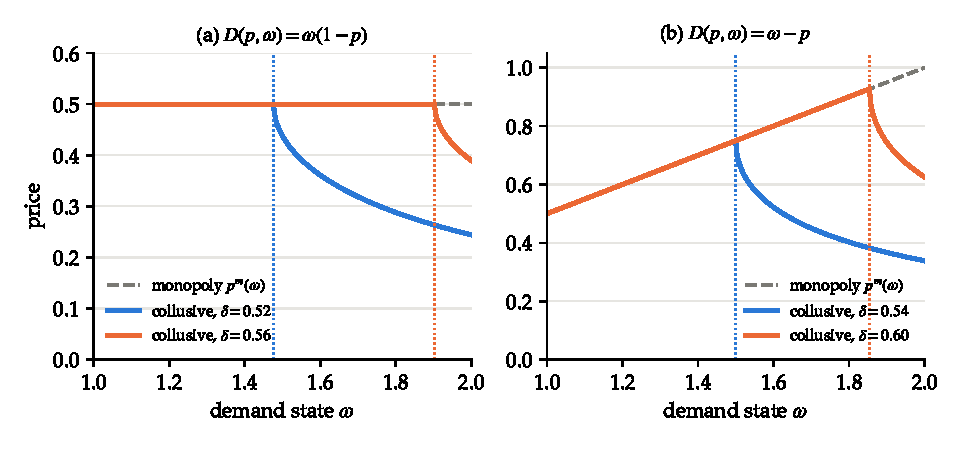
\includegraphics[width=\textwidth]{figures/ch12/rs_continuum.pdf}
\caption{Most collusive price schedules with observable independent demand shocks: $N = 2$, $c = 0$,
$\omega \sim U[1,2]$. Panel (a): multiplicative shocks, $D(p,\omega) = \omega(1-p)$. Panel (b): additive shocks,
$D(p,\omega) = \omega - p$. Dashed: monopoly price $p^m(\omega)$. Solid: collusive price $p^*(\omega)$ for two discount
factors. Dotted vertical lines mark the cutoffs $\omega^*$ of \cref{prop:12-rs-threshold}. Below the cutoff the
collusive price equals the monopoly price. Above it, profit is capped at $\kappa E^*$ and the price falls as demand
rises. Script \texttt{rs\_continuum.py}.}
\label{fig:12-rs-continuum}
\end{figure}

\subsubsection{Collude or compete}

In the optimal scheme no price war is ever observed. The cartel lowers its price smoothly in booms. The paper
also studies a simpler set of strategies in which the cartel can only choose between the monopoly price and the
competitive price (p.~12). Such strategies are ``much simpler and less delicate.'' With this restriction ``the firms
know that when demand is high the monopoly outcome cannot be maintained. They therefore assume that the competitive
outcome will emerge, which is sufficient to fulfill their prophecy.''

Formally, a \emph{collude-or-compete scheme} charges $p^m(\omega)$ in a set $C$ of states and $c$ outside it. In states
outside $C$ all firms charge $c$, a static Nash equilibrium, so nobody wants to deviate there. In a state
$\omega \in C$ the incentive constraint is $\pi^m(\omega) \le \kappa E_R$, where $E_R = \E[\pi^m(\omega)\indic\{\omega \in C\}]$.
Including a low state in $C$ raises $E_R$ without raising the largest profit to be protected. So the best set is an
interval $[\underline\omega, x]$, and the scheme is sustainable if and only if
\begin{equation}\label{eq:12-rs-restricted}
\pi^m(x) \le \kappa\int_{\underline\omega}^{x}\pi^m(\omega)\, \dd F_\omega(\omega).
\end{equation}
A sustainable collude-or-compete scheme is also sustainable in the unrestricted problem. So $E_R \le E^*$, and when
$x$ is interior, $\pi^m(x) \le \kappa E_R \le \kappa E^* = \pi^m(\omega^*)$, so $x \le \omega^*$. The cartel colludes in
fewer states than under the optimal scheme, as the paper states. Above $x$ the price drops from $p^m(x)$ to $c$: an
outright price war, triggered by high demand. This version is the one that connects with empirical studies that
classify periods as collusive or competitive, such as \citet{Bresnahan1987} and \citet{Porter1983}.

\begin{remark}[When do collude-or-compete schemes produce wars?]\label{rem:12-rs-restricted}
Condition \eqref{eq:12-rs-restricted} can fail for every interior $x$ even when the optimal scheme sustains a lot of
collusion. In the two-state model, colluding only in the low state requires $\pi_L^M \le \kappa\cdot\frac{1}{2}\pi_L^M$,
that is $\kappa \ge 2$. But $\bar\kappa < 2$, so for $\kappa \ge 2$ the cartel can already charge monopoly prices in
both states. The restricted scheme is all or nothing. The same happens in both examples of \cref{fig:12-rs-continuum}.
Our computation gives $E_R = 0$ at all four discount factors shown, although the optimal scheme earns between 82 and
almost 100 percent of expected monopoly profit there. The right side of \eqref{eq:12-rs-restricted} is small for $x$ near
$\underline\omega$. A war region at the top therefore requires a distribution in which very high states are rare. Then
the low states accumulate enough profit to protect collusion up to some $x$, and the thin upper tail adds too little
to protect collusion beyond it.
\end{remark}

The shares in the remark are $\frac{0.341}{0.375} \approx 0.91$ and $\frac{0.374}{0.375} \approx 0.997$ in panel (a), and
$\frac{0.479}{0.583} \approx 0.82$ and $\frac{0.573}{0.583} \approx 0.98$ in panel (b).

\subsubsection{Increasing marginal cost}

The model so far assumes constant marginal cost. Increasing marginal cost complicates the model in three ways
(p.~12). First, a price cutter may not want to supply all demand at its price, since it never produces where marginal
cost exceeds price. Second, the profit that the cartel can sustain differs across states, unlike in the constant-cost
case. Third, cheating can take the form of raising price, since rivals that are unwilling to supply all demand at
their price leave some customers for a firm that charges more.

When deviators do not meet all demand, the paper uses the envelope theorem (p.~13). Suppose first that the cartel
charges the monopoly price, which rises with demand. A deviator produces its output $q^d$ where marginal cost equals
the collusive price. By the envelope theorem its profit rises with the state at rate
$q^d\frac{\partial P}{\partial \omega}$, where $P$ is inverse demand. A conforming firm's profit rises at the smaller
rate $q^m\frac{\partial P}{\partial \omega}$, because $q^m < q^d$. Deviation therefore becomes more tempting as demand
rises. Suppose instead that the cartel holds its price fixed as demand rises. The deviation profit then stays fixed.
The conforming profit rises, because the collusive price exceeds marginal cost, and the temptation falls.

When deviators meet all demand, the paper works with the linear example
\begin{equation}\label{eq:12-rs-linear}
P = a + \omega - bQ, \qquad C(q_i) = c\,q_i + \frac{d}{2}q_i^2,
\end{equation}
where $Q$ is industry output and $C$ is each firm's cost (eqs.~(6) and (7)). A cartel that splits output equally
maximizes $(a + \omega - bQ)Q - cQ - \frac{d}{2N}Q^2$. The first-order condition $a + \omega - 2bQ - c - \frac{d}{N}Q = 0$
gives monopoly output and price (eqs.~(8) and (9)):
\begin{equation*}
Q^m = \frac{a + \omega - c}{2b + \frac{d}{N}}, \qquad
P^m = a + \omega - bQ^m = \frac{(a+\omega)(bN + d) + bNc}{2bN + d}.
\end{equation*}
A deviator charging just below $P^m$ would like to produce where $c + dq = P^m$, that is
\begin{equation*}
\bar q = \frac{P^m - c}{d} = \frac{(a + \omega - c)\left(b + \frac{d}{N}\right)}{d\left(2b + \frac{d}{N}\right)}
\end{equation*}
(eq.~(10)). Dividing, $\frac{\bar q}{Q^m} = \frac{b + \frac{d}{N}}{d}$. The deviator meets all demand if and only if
$\bar q \ge Q^m$, that is $b \ge \frac{(N-1)d}{N}$. Marginal cost must not rise too steeply and $N$ must not be too large.
When the deviator meets demand, it sells $Q^m$ at $P^m$ alone, so
\begin{equation*}
\Pi^d = P^mQ^m - cQ^m - \frac{d}{2}(Q^m)^2 .
\end{equation*}
Per-firm collusive profit is $\Pi^m = \frac{1}{N}(P^mQ^m - cQ^m) - \frac{d}{2}\left(\frac{Q^m}{N}\right)^2$. Hence
\begin{equation*}
\Pi^d - N\Pi^m = -\frac{d}{2}(Q^m)^2 + \frac{d}{2N}(Q^m)^2 = \frac{Nd(1-N)}{2}(q^m)^2, \qquad q^m = \frac{Q^m}{N},
\end{equation*}
which is eq.~(11). By the envelope theorem, $\frac{\dd\Pi^m}{\dd\omega} = q^m$. Since $\Pi^d - \Pi^m = (N-1)\Pi^m +
\frac{Nd(1-N)}{2}(q^m)^2$ and $\frac{\dd q^m}{\dd\omega} = \frac{1}{2bN + d}$,
\begin{equation}\label{eq:12-rs-incmc}
\frac{\dd(\Pi^d - \Pi^m)}{\dd\omega} = (N-1)q^m - Nd(N-1)\frac{q^m}{2bN + d} = \frac{(N-1)q^m\left(2bN - d(N-1)\right)}{2bN + d},
\end{equation}
which is eq.~(12). It is positive whenever the deviator meets demand, because then $2bN \ge 2d(N-1) > d(N-1)$. Cheating
becomes more attractive as demand rises.

The paper computes the optimal schedule numerically. For a given punishment, the sustainable price in each state
solves a quadratic equation. The punishment is then updated, starting from a large value and iterating to the first
fixed point (p.~14). Its Figure 1 uses $a = 60$, $b = 1$, $c = 0$, $d = \frac{1}{3}$, $\delta = 0.7$, $N = 5$ and a state
uniform on $\{0, 1, \dots, 80\}$. By eq.~(9) the monopoly price rises linearly from about $30.97$ in state $0$ to about
$72.26$ in state $80$ (our computation). The collusive price equals the monopoly price only in the lowest states. It
then falls, reaches a minimum in the middle of the range of states, and rises slowly at high states. The rise at the
top has a simple cause (p.~15). In high states the collusive price is so low that a deviator would expand only until
price equals its marginal cost. It would no longer serve the whole market. From there, higher demand at a constant
price reduces the temptation, ``thus the oligopoly can afford to increase its prices somewhat.''

\subsubsection{Quantity competition}

With quantities as strategic variables two things change (p.~15). A deviator takes rivals' outputs as given, so its
residual demand is market demand shifted left by their combined output. And the punishment is the Cournot
equilibrium, which yields positive profit. The results are weaker than with prices. Higher demand need not raise the
temptation to cheat. The paper gives a counterexample (p.~16 and its Figure 2). Suppose demand has constant elasticity
and a shock shifts it horizontally. Then the collusive price is the same in both states, and a deviator faces the same
residual demand curve in both, up to a horizontal translation. The extra sales from cheating are the same in both
states, but the revenue lost on the units it would have sold anyway is smaller in the low state. So the incentive to
deviate is strictly larger in the low state. The authors draw a related conclusion: if the cartel keeps its price
constant when demand shifts horizontally, the incentive to cheat falls.

A short calculation makes the counterexample precise. Let marginal cost be a constant $c$, and let $\bar p$ be the
collusive price in both states. In the high state $\omega''$ demand exceeds demand in the low state $\omega'$ by a
constant $k > 0$ at every price. Each firm's collusive output is $q^s(\omega) = \frac{1}{N}D(\bar p,\omega)$, so
$q^s(\omega'') > q^s(\omega')$. Rivals keep producing $(N-1)q^s(\omega)$. A deviator that charges $p < \bar p$
therefore sells $D(p,\omega) - (N-1)q^s(\omega) = q^s(\omega) + y(p)$. The extra sales
$y(p) = D(p,\omega) - D(\bar p,\omega)$ are the same in both states, because the shift $k$ cancels. The deviator's
gain over its conforming profit $\Pi^s(\omega) = (\bar p - c)\,q^s(\omega)$ is
\begin{equation*}
\begin{aligned}
\Pi^d(p,\omega) - \Pi^s(\omega)
&= (p - c)\bigl[q^s(\omega) + y(p)\bigr] - (\bar p - c)\,q^s(\omega) \\
&= (p - c)\,y(p) - (\bar p - p)\,q^s(\omega) .
\end{aligned}
\end{equation*}
The first term is the profit on the extra sales, the equal segments AB and CD of the paper's Figure 2 (p.~16). The
second term is the loss on the units the firm would have sold anyway, and it rises with $q^s(\omega)$. Hence every
deviation price $p < \bar p$ gains strictly more in the low state. If some deviation pays in the high state, the best
deviation pays strictly more in the low state.

With linear demand and cost \eqref{eq:12-rs-linear}, higher demand always raises the temptation. Suppose each firm is
asked to produce $q^s$. A deviator maximizes (eq.~(13))
\begin{equation*}
\Pi^d = q_i\left[a + \omega - c - b\left((N-1)q^s + q_i\right)\right] - \frac{d}{2}q_i^2 ,
\end{equation*}
and the first-order condition gives (eq.~(14))
\begin{equation*}
q^d = \frac{a + \omega - c - b(N-1)q^s}{2b + d} .
\end{equation*}
Let $X = a + \omega - c$ and evaluate at the monopoly output $q^s = q^m = \frac{X}{2bN + d}$. The term in brackets of the
deviator's problem is $A \equiv X - b(N-1)q^m = \frac{X(bN + b + d)}{2bN + d}$, and the deviator earns
$\Pi^d = \frac{A^2}{2(2b + d)}$. A conforming firm earns $\Pi^m = q^m(X - bNq^m) - \frac{d}{2}(q^m)^2 = \frac{X^2}{2(2bN + d)}$.
Subtracting, and using $(bN + b + d)^2 - (2b+d)(2bN + d) = b^2(N-1)^2$,
\begin{equation*}
\Pi^d - \Pi^m = \frac{b^2(N-1)^2 X^2}{2(2b+d)(2bN+d)^2}, \qquad
\frac{\dd(\Pi^d - \Pi^m)}{\dd\omega} = \frac{\left[b(N-1)\right]^2(a + \omega - c)}{(d + 2bN)^2(2b + d)} > 0 .
\end{equation*}
The derivative is the expression on p.~17 of the paper. If the cartel can only collude or compete, high states produce
price wars. If it can choose output freely, it raises output in high states just enough to deter deviation. The
paper's Figure 3 uses $a = 60$, $b = 1$, $c = 0$, $d = \frac{1}{3}$, $\delta = 0.7$ and $N = 5$, the parameters of its
Figure 1. It plots the ratio of the collusive to the monopoly price. The ratio equals one in states up to about 61 and
then falls almost linearly to about $0.92$ in state $80$ (values read from the figure).
The figure's axis is labeled ``Monopoly Price/Oligopoly Price,'' but the text and the plotted values below one
show that it is the oligopoly price relative to the monopoly price. These quantity results hold within Nash-reversion
punishments. In the Cournot supergame harsher credible punishments exist (\cref{sec:12-perfect}), and with them the
cap would be higher.

\subsubsection{From oligopoly pricing to business cycles}

The paper's Section III embeds the oligopoly in a two-sector general equilibrium model (pp.~19--23). Sector 1 is
competitive and sector 2 is the oligopoly. Workers supply any amount of labor at a wage equal to the price of good 1,
and both are normalized to one. Good 1 is produced from labor $L_{1t}$ and an input $Q_{21t}$ of good 2 (p.~19),
\begin{equation}\label{eq:12-rs-ge-prod}
Q_{1t} = A_1Q_{21t} - \frac{B_1}{2}Q_{21t}^2 + G_1L_{1t} - \frac{H_1}{2}L_{1t}^2 .
\end{equation}
Competitive firms equate the price of each input with its marginal revenue product. For good 2 this gives the input
demand
\begin{equation*}
P_{2t} = A_1 - B_1Q_{21t}
\quad\Longleftrightarrow\quad
Q_{21t} = \frac{A_1 - P_{2t}}{B_1} .
\end{equation*}
For labor it gives $G_1 - H_1L_{1t} = 1$, so employment in sector 1 is constant. Consumers' inverse demand for good 2
is $P_{2t} = A_c - B_cQ_{2ct} + e_t$, where $e_t$ is an \iid\ taste shock. Add the two demands,
$Q_{2t} = Q_{21t} + Q_{2ct}$, and solve for $P_{2t}$:
\begin{equation*}
P_{2t} = a + \omega_t - bQ_{2t},
\qquad
a = \frac{A_cB_1 + B_cA_1}{B_c + B_1},
\quad
b = \frac{B_cB_1}{B_c + B_1},
\quad
\omega_t = \frac{B_1}{B_c + B_1}\,e_t .
\end{equation*}
This is the linear demand of \eqref{eq:12-rs-linear}. Producing $Q_{2t}$ requires $cQ_{2t} + \frac{d}{2}Q_{2t}^2$ units of
labor, so marginal cost is $c + dQ_{2t}$ as in the partial-equilibrium model (p.~20).\footnote{Rotemberg and Saloner
write $\alpha$, $\beta$, $\gamma$, $\xi$, $n$, $m$ and $\varepsilon_t$ for our $A_1$, $B_1$, $G_1$, $H_1$, $A_c$, $B_c$ and
$\omega_t$. Their equations (14) and (16) on pp.~19--20 print the labor demand as $\frac{1 + \gamma}{\xi}$ and the
intercept as $\frac{n\beta + m\gamma}{m + \beta}$. The first-order conditions give $\frac{\gamma - 1}{\xi}$ and
$\frac{n\beta + m\alpha}{m + \beta}$. Neither difference affects the argument. The working paper's numbers (13) and
(14) for these equations repeat numbers already used on p.~17, so we cite the section by page.}

The two outputs are linked through the price of good 2. Differentiate \eqref{eq:12-rs-ge-prod} along the input demand:
\begin{equation*}
\frac{\partial Q_{1t}}{\partial P_{2t}}
= \bigl(A_1 - B_1Q_{21t}\bigr)\frac{\partial Q_{21t}}{\partial P_{2t}}
= P_{2t}\cdot\Bigl(-\frac{1}{B_1}\Bigr) < 0 .
\end{equation*}
Output of good 2 is $Q_{2t} = \frac{a + \omega_t - P_{2t}}{b}$, which rises with $\omega_t$ and falls with $P_{2t}$.
Suppose first that sector 2 is competitive, or always acts as a monopolist. Both the competitive and the monopoly
price rise with $\omega_t$, so a taste shift toward good 2 lowers the output of good 1 (p.~20). The two outputs move
in opposite directions, and the economy moves along a production possibility frontier. Suppose instead that the
oligopoly plays the optimal supergame with prices as the strategic variable. A higher $\omega_t$ can then lower
$P_{2t}$ (\cref{sec:12-rs}). Sector 1 buys more of the input and expands, and sector 2 sells more as well. Both
outputs rise together, as all outputs do in a boom (p.~21). Profits can still be procyclical, because revenue minus
total cost can rise with output when there are fixed costs, even as margins fall (p.~22). The authors argue that
this mechanism makes sticky prices and a multiplier natural. They also argue that stabilization
policy could be harmful if booms reflect shifts toward oligopolistic goods. ``If demand for the goods produced by
oligopolies were stable they might collude always, leaving the economy in a permanent recession'' (p.~37).

\subsubsection{The evidence}

Section IV of the paper confronts the folklore with four kinds of evidence (pp.~24--36). None of them is a structural
test. Each asks whether prices or margins in concentrated industries fall when demand is high.

\casehead{The folklore}
\citet{Scherer1980} cites three industries in support of the folklore: rayon, cement and steel. The rayon evidence
shows mainly that the nominal price of rayon fell in the Great Depression, when broad price indices also fell. That
is ``hardly proof of a price war'' (p.~24). For steel, Scherer himself grants that the industry avoided ``widespread
price deterioration, even when operating at less than 65\% capacity between 1958 and 1962'' (p.~24). That leaves
cement.

\casehead{Cement: data and estimating equation}
The data are yearly from 1947 to 1981. The cement price $p^c_t$ is the average price of portland cement from the
Bureau of Mines' \textit{Minerals Yearbook}. It is deflated either by the producer price index $\mathit{PPI}_t$ or by the
price index of construction materials $p^{\mathit{con}}_t$, both from the Bureau of Labor Statistics. The regression
relates the yearly growth rate of the real cement price to the contemporaneous growth rate of GNP. In log-difference
notation,
\begin{equation}\label{eq:12-rs-cement}
\Delta \ln\left(\frac{p^c_t}{P_t}\right) = \beta_0 + \beta_1\, \Delta\ln \mathit{GNP}_t + u_t, \qquad u_t = \phi\, u_{t-1} + e_t,
\qquad P_t \in \left\{\mathit{PPI}_t,\ p^{\mathit{con}}_t\right\}.
\end{equation}
The paper describes the variables as yearly growth rates and does not say whether they are log differences or
percentage changes. Columns (1) and (3) of its Table 1 are ordinary least squares with $\phi = 0$. The Durbin-Watson
statistics of these regressions are low, so columns (2) and (4) re-estimate the equation with first-order
autoregressive errors, ``quasi-differenced'' in the paper's words (p.~25). The paper does not say which feasible
generalized least squares procedure it uses.

The identifying assumption is that GNP growth shifts the demand for cement and is unrelated to the cost and capacity
shocks of the cement industry. The theory predicts $\beta_1 < 0$: when demand grows faster, the collusive price falls
relative to other prices. A competitive industry with rising marginal cost, or a monopoly with procyclical monopoly
prices, would instead show $\beta_1 \ge 0$.

\begin{table}[htbp]
\centering
\caption{The cyclical behavior of real cement prices, yearly data 1947--1981}\label{tab:12-rs-cement}
\small
\begin{tabular}{@{}lcccc@{}}
\toprule
 & (1) & (2) & (3) & (4)\\
Dependent variable: growth of & $\frac{p^c}{\mathit{PPI}}$ & $\frac{p^c}{\mathit{PPI}}$ & $\frac{p^c}{p^{\mathit{con}}}$ & $\frac{p^c}{p^{\mathit{con}}}$\\
\midrule
Constant & 0.025 & 0.025 & 0.038 & 0.037\\
 & (0.010) & (0.012) & (0.007) & (0.008)\\[2pt]
GNP growth, $\beta_1$ & $-0.438$ & $-0.456$ & $-0.875$ & $-0.876$\\
 & (0.236) & (0.197) & (0.161) & (0.149)\\[2pt]
AR(1) coefficient, $\phi$ & & 0.464 & & 0.315\\
 & & (0.173) & & (0.183)\\[2pt]
$R^2$ & 0.10 & 0.15 & 0.48 & 0.52\\
Durbin-Watson & 1.03 & 1.73 & 1.28 & 1.92\\
\bottomrule
\end{tabular}

\smallskip
\begin{minipage}{0.86\textwidth}
\footnotesize
Notes: Estimates of \eqref{eq:12-rs-cement}. $p^c$ is the price of cement, $\mathit{PPI}$ the producer price index and
$p^{\mathit{con}}$ the price index of construction materials. Columns (1) and (3) are ordinary least squares. Columns (2)
and (4) allow first-order autocorrelated errors and are estimated on quasi-differenced data. Standard errors in
parentheses. The paper reports no sample size. Yearly data for 1947--1981 give at most 35 growth rates. Source:
\citet{RotembergSaloner1984}, Table 1.
\end{minipage}
\end{table}

\casehead{Cement: results}
\Cref{tab:12-rs-cement} shows a negative coefficient on GNP growth in all four columns. ``A 1\% increase in the rate of
growth of GNP leads to a 0.5--1.0\% fall in the price of cement'' (p.~25). After the correction for autocorrelation the
coefficients are significant at the 5 percent level. The $t$-ratios are $\frac{-0.456}{0.197} \approx -2.3$ in column (2)
and $\frac{-0.876}{0.149} \approx -5.9$ in column (4). The ordinary least squares standard errors in columns (1) and (3)
are not reliable given the low Durbin-Watson statistics. The anecdotes agree. The real price of cement rose in the
recession years 1954 and 1958 and fell in the boom years 1955 and 1959 (p.~25).

\casehead{Cement: caveats}
The authors raise two objections themselves (pp.~25--26). First, the demand for cement might be only weakly related
to GNP. Cement output growth has a correlation of $0.69$ with GNP growth and $0.77$ with the growth of construction,
which is procyclical. These correlations do not show that cement is more cyclical than the typical sector in GNP.
Without a structural model the question cannot be settled. Second, the regression omits variables a reduced form
should contain, such as the capacity of cement plants. The authors reply that capacity is endogenous and that
adjustment costs make it unresponsive to GNP in the short run. Three further concerns are worth stating. Input costs,
such as energy prices in the 1970s, may move against GNP and enter the cement price directly. If the
construction-materials index in columns (3) and (4) is procyclical, the deflated price is mechanically more
countercyclical, which may explain why those coefficients are larger. And a negative
$\beta_1$ is consistent with any model in which margins fall in booms, including models with capacity constraints or
countercyclical demand elasticities. The regression supports the prediction without isolating the mechanism.

\casehead{Railroads in the 1880s}
\citet{Porter1983} estimated when the railroad cartel on the route from Chicago to New York, the Joint Executive
Committee, was colluding and when it was in a price war. Green and Porter's theory predicts wars after unexpectedly low demand.
Rotemberg and Saloner say that Porter ``finds no support for this theory from the residuals of his estimated
equations'' and argue that his results support their theory instead (p.~26). \Cref{tab:12-rs-railroads} reproduces
their evidence. The first three columns come from Porter's paper. The first is Porter's estimated index of cartel
nonadherence, which parallels closely the contemporary reports in the \textit{Railway Review} and the
\textit{Chicago Tribune}. The second gives rail shipments of wheat from Chicago to New York. The third gives the share
of wheat shipped from Chicago by rail rather than by lake. The last two columns are from the Chicago Board of Trade
annual reports. National grain production adds wheat, corn, rye, oats and barley in tons. The last column counts the
days between April 1 and December 31 on which the Straits of Mackinac were closed to navigation, which prevented
shipment by lake.

\begin{table}[htbp]
\centering
\caption{The railroad cartel, 1880--1886}\label{tab:12-rs-railroads}
\small
\setlength{\tabcolsep}{3pt}
\begin{tabular}{@{}lccccc@{}}
\toprule
 & Estimated & Rail shipments & Fraction shipped & Total grain production & Days lakes closed\\
Year & nonadherence & (million bushels) & by rail (\%) & (billion tons) & (April 1 to Dec.\ 31)\\
\midrule
1880 & 0.00 & 4.73 & 22.1 & 2.70 & 35\\
1881 & 0.44 & 7.68 & 50.0 & 2.05 & 69\\
1882 & 0.21 & 2.39 & 13.8 & 2.69 & 35\\
1883 & 0.00 & 2.59 & 26.8 & 2.62 & 58\\
1884 & 0.40 & 5.90 & 34.0 & 2.98 & 58\\
1885 & 0.67 & 5.12 & 48.5 & 3.00 & 61\\
1886 & 0.06 & 2.21 & 17.4 & 2.83 & 50\\
\bottomrule
\end{tabular}

\smallskip
\begin{minipage}{0.92\textwidth}
\footnotesize
Notes: Columns 1 to 3 are from \citet{Porter1983}, columns 4 and 5 from the Chicago Board of Trade annual reports,
as compiled by Rotemberg and Saloner. Units as printed in the source. The lakes were always closed from January 1 to
March 31. Source: \citet{RotembergSaloner1984}, Table 2.
\end{minipage}
\end{table}

The most severe price wars occurred in 1881, 1884 and 1885. These are the years with the largest rail shipments, in
absolute terms and relative to lake shipments (p.~27). This alone does not show high demand, since shipments may be
high because railroads compete. The authors therefore look at two determinants of demand for rail transport. The
lakes stayed closed longest in 1881 and 1885, the years with the highest nonadherence. In 1883 and 1884 the lakes
were closed only slightly less than in 1885, yet there was a war only in 1884. Grain production explains 1883. It was
the second lowest of the period and 12 percent below 1884 (p.~28). In the authors' words, this ``must have depressed
demand so much that, in spite of the lake closings, total demand for rail transport was low enough to warrant
cooperation.''

The authors anticipate two objections (pp.~28--29). Porter used weekly data, while their table is annual. They reply
that the wars followed a seasonal pattern. The first began around January 1881 and lasted the whole year. The second
began around January 1884 and ended at the end of 1885. Agents could predict the opening of the lakes in midwinter by
studying the thickness of the ice. A railroad that expected a war in the future had two reasons to cut its price at
once. The penalty for deviating was smaller, since the future would be competitive anyway. And shippers who could store
grain would postpone shipments ahead of an expected war, which lowered even the monopoly price. The second objection is
that national grain production is a poor proxy for production in the Chicago region. They reply that national
movements mostly reflect the grain belt, which includes Illinois. The weekly analysis belongs to Porter's own paper and
to \citet{Ellison1994}, who tests Green-Porter against Rotemberg-Saloner with the same data. \Cref{sec:13-jec}
treats both.

\casehead{Automobiles in 1955}
\citet{Bresnahan1987} studies the American automobile industry in the model years 1954 to 1956 (\cref{sec:06-bresnahan}).
Production in 1955 was 44 percent above its 1954 level, and it fell by about 27 percent in 1956
(\cref{tab:06-bres-facts}). The working paper of \citet{RotembergSaloner1984} reports a 45 percent rise and a 44
percent fall (p.~26). The second figure does not match Bresnahan's Table I. Bresnahan finds that a model of
competitive pricing fits the 1955 data, while a collusive model fits 1954 and 1956. Rotemberg and Saloner add that GNP
fell 1 percent in 1954, rose 7 percent in 1955 and rose 2 percent in 1956 (p.~26). In their words, ``Insofar as
cartels can only sustain either competitive or collusive outcomes, this is what our theory predicts'' (p.~26). The
competitive year was the boom year.

\casehead{Price-cost margins}
A direct test would compare prices with marginal costs in booms and recessions. Marginal cost data are scarce, so
industrial organization economists use the \emph{price-cost margin}, sales minus payroll and material costs, divided by
sales. \citet{Scherer1980} summarizes the studies of its cyclical behavior (his p.~357, quoted on p.~29). Concentrated
industries reduce prices, and above all price-cost margins, ``by less in response to a demand slump and increase them
by less in the boom phase.'' The folklore predicts the opposite. Rotemberg and Saloner argue that the fact
favors their theory (p.~30). If part of payroll is a fixed cost, measured margins rise in booms even when price and
marginal cost do not change. Measured margins in concentrated industries rise by less. Either fixed costs matter less
in concentrated industries, which they find unlikely, or concentrated industries cut prices relative to marginal cost
in booms.

\casehead{Product wages and concentration}
The last piece of evidence uses correlations between employment and the \emph{real product wage}. This is the average
hourly wage divided by the industry's value-added deflator. \citet{Burda1984} computed the correlations from detrended
yearly data for 1947--1978. To see why it measures margins, let marginal cost be $mc = \frac{w}{MPL}$, where $w$ is the wage and $MPL$
the marginal product of labor. Then
\begin{equation*}
\frac{w}{p} = MPL \cdot \frac{mc}{p} = MPL\,(1 - L),
\end{equation*}
with $L$ the Lerner index. With constant marginal product, a product wage that rises with employment means a Lerner
index that falls in booms. With diminishing returns, $MPL$ falls in booms, which strengthens the inference (p.~31). The
measure remains valid when part of payroll is fixed. Its weakness is that materials must be proportional to output and
passed through as in a competitive industry (p.~30). The concentration ratio of each two-digit industry is a 1967
sales-weighted average of four-digit four-firm ratios.

\begin{table}[htbp]
\centering
\caption{Concentration and the correlation between real product wages and employment}\label{tab:12-rs-wages}
\small
\setlength{\tabcolsep}{5pt}
\begin{tabular}{@{}llcccc@{}}
\toprule
\multicolumn{6}{@{}l}{\textit{Panel A: two-digit manufacturing industries}}\\
SIC & Industry & Correlation & CR4 & Group & Sign\\
\midrule
\multicolumn{6}{@{}l}{Durables}\\
24 & Lumber and wood products & $-0.33$ & 17.6 & U & $-$\\
25 & Furniture and fixtures & $-0.18$ & 21.6 & U & $-$\\
32 & Stone, clay and glass & 0.39 & 37.4 & C & $+$\\
33 & Primary metals & 0.32 & 42.9 & C & $+$\\
34 & Fabricated metal industries & 0.23 & 29.1 & U & $+$\\
35 & Machinery except electrical & 0.12 & 36.3 & C & $+$\\
36 & Electrical and electronic equipment & 0.34 & 45.0 & C & $+$\\
371 & Motor vehicles and equipment & 0.19 & 80.8 & C & $+$\\
372--9 & Other transportation equipment & 0.02 & 50.1 & C & $+$\\
38 & Instruments and related products & $-0.36$ & 47.8 & C & $-$\\[2pt]
\multicolumn{6}{@{}l}{Nondurables}\\
20 & Food and kindred products & $-0.30$ & 34.5 & U & $-$\\
21 & Tobacco manufactures & $-0.64$ & 73.6 & C & $-$\\
22 & Textile mill products & 0.04 & 34.1 & U & $+$\\
23 & Apparel and related products & $-0.53$ & 19.7 & U & $-$\\
26 & Paper and allied products & $-0.42$ & 31.2 & U & $-$\\
27 & Printing and publishing & 0.40 & 18.9 & U & $+$\\
28 & Chemical and allied products & $-0.03$ & 49.9 & C & $-$\\
29 & Petroleum and coal products & $-0.48$ & 32.9 & U & $-$\\
30 & Rubber & 0.16 & 69.1 & C & $+$\\
31 & Leather and leather products & $-0.44$ & 24.5 & U & $-$\\
\midrule
\multicolumn{6}{@{}l}{\textit{Panel B: contingency table}}\\
 & & Unconcentrated (U) & Concentrated (C) & Total & \\
\midrule
\multicolumn{2}{@{}l}{Negatively correlated} & 7 & 3 & 10 & \\
\multicolumn{2}{@{}l}{Positively correlated} & 3 & 7 & 10 & \\
\multicolumn{2}{@{}l}{Total} & 10 & 10 & 20 & \\
\bottomrule
\end{tabular}

\smallskip
\begin{minipage}{0.9\textwidth}
\footnotesize
Notes: ``Correlation'' is the correlation between the real product wage and employment, detrended yearly data
1947--1978, from \citet{Burda1984}. CR4 is the 1967 four-firm concentration ratio, a sales-weighted average over
four-digit industries (excluding those ending in 99). The groups split the sample at the median concentration of 35.4.
The Group and Sign columns are our classification, and they reproduce Panel B. Source: \citet{RotembergSaloner1984},
Tables 3 and 4.
\end{minipage}
\end{table}

Panel A of \cref{tab:12-rs-wages} shows that concentrated industries such as motor vehicles and electrical equipment
tend to have positive correlations. Unconcentrated ones such as leather, food and wood products tend to have negative
correlations (p.~32). The theory does not say that a slightly more concentrated industry cuts prices more in
booms. A pure monopoly charges the monopoly price, which usually rises with demand. So the authors split the sample at
the median concentration ratio of 35.4, which lies between food and nonelectrical machinery. Panel B gives the
resulting $2 \times 2$ table. Dropping the three industries whose correlations are close to zero (SIC 22, 28 and
372--9) turns the counts 7:3:3:7 into 7:2:2:6. A $\chi^2$ test rejects independence with 92 percent confidence for
Panel B and 97 percent for the reduced table. Fisher's exact test against the alternative that concentrated industries
have more positive correlations rejects with 91 and 96 percent confidence (pp.~33--34). We recomputed these numbers.
The Pearson statistic without continuity correction is $3.20$ ($p = 0.074$) for Panel B and $4.74$ ($p = 0.030$) for the
reduced table. The one-sided Fisher $p$-values are $0.089$ and $0.045$.

\casehead{Alternative explanations}
The authors discuss two (p.~34). Positive correlations could come from monopoly pricing with short-run increasing
returns to labor. They find this unlikely, because firms cut production by closing their least efficient plants
first. Positive correlations could also come from technology shocks that raise labor demand in a sector with upward
sloping labor supply. But the sectors with positive correlations, such as stone, clay and glass, printing and
publishing, and rubber, ``appear to be sectors with fairly stagnant technologies'' (p.~35).

\subsubsection{Critiques and limitations}

The theory and the evidence have limits that later work addressed.
\begin{enumerate}[label=(\arabic*)]
\item \emph{Selection and patience.} Countercyclical pricing describes the most collusive equilibrium for intermediate
discount factors. The competitive equilibrium and many constant-price equilibria exist as well. The theory restricts
what can be sustained, and the prediction rests on the selection.
\item \emph{Independent shocks.} Business cycles are persistent. A boom today predicts high demand tomorrow, which
raises the future loss from a price war exactly when the current gain is large. \Cref{sec:12-hh,sec:12-bs} show
that persistence can reverse the prediction. \citet{Kandori1991} shows that countercyclical pricing survives a family
of correlated shocks when the discount factor is close to a specific value determined by $N$, as summarized by
\citet[p.~2]{BagwellStaiger1995}.
\item \emph{No wars on the path.} With observable demand the optimal scheme lowers prices smoothly. Actual breakdowns
need restricted strategies, and \cref{rem:12-rs-restricted} shows that even then wars at the top require special
distributions. Wars that follow unobserved shocks belong to the theory of \cref{sec:12-public}.
\item \emph{Other forces.} \citet{StaigerWolak1992} add capacity constraints to the model. As Bagwell and Staiger
summarize it, low prices may then be required during downturns, a conclusion analogous to Green and Porter's
\citep[fn.~1]{BagwellStaiger1995}. Storage and intertemporal substitution by buyers, which the authors invoke for the
railroads, also change the incentive constraints.
\item \emph{Reduced-form evidence.} Each piece of evidence shows that margins or prices fall in booms in concentrated
industries. None identifies the mechanism. Capacity, input costs, demand elasticities and fixed costs can produce the
same correlations. The classification by concentration is crude, as the authors note for printing. Its concentration
ratio is low, but its main components, newspapers, books and magazines, are highly concentrated once location and
type are taken into account (p.~32).
\end{enumerate}

\subsubsection{The link to conduct estimation}

Rotemberg-Saloner collusion makes conduct vary with demand. This matters for the conduct-parameter method of
\cref{ch:conduct}. Write the supply relation as
\begin{equation*}
p_t - c_t = \theta_t m_t, \qquad m_t = \frac{Q_t}{\left|\frac{\partial Q_t}{\partial p_t}\right|},
\end{equation*}
where $m_t$ is the markup term. Suppose conduct falls linearly with demand, $\theta_t = \vartheta_0 - \vartheta_1 m_t$
with constants $\vartheta_0$ and $\vartheta_1 > 0$, as in a cartel that concedes in booms. A researcher who estimates
a constant conduct parameter by instrumental variables with a demand shifter recovers a weighted average of the local
slope of the supply relation (\cref{prop:03-corts}). The markup is
$\theta_t m_t = \vartheta_0 m_t - \vartheta_1 m_t^2$, whose slope is $\vartheta_0 - 2\vartheta_1 m_t$. For small
demand movements around $\bar m$ the estimate is close to $\vartheta_0 - 2\vartheta_1\bar m$, while average conduct is
$\vartheta_0 - \vartheta_1\bar m$. The estimate understates market power and can be
negative \citep{Corts1999}. \Cref{sec:03-corts} develops the general result.

\subsubsection{Contribution}

The paper made three lasting contributions. It gave a general logic for collusion under fluctuating demand: compare
the current temptation with the expected future loss, and adjust the collusive price state by state to balance them.
It derived a testable prediction about markups over the cycle, the opposite of the folklore. And it reinterpreted
observed price wars, such as those of 1955 and the 1880s, as consequences of high demand. The papers in the rest of
this section keep the logic and change the demand process.

\subsection{Predictable cycles: Haltiwanger and Harrington (1991)}\label{sec:12-hh}

\citet{HaltiwangerHarrington1991} replace independent shocks with a deterministic demand cycle that firms know in
advance. The original paper is not available to us. We describe its results as \citet[pp.~1--3]{BagwellStaiger1995}
summarize them and develop the logic in our own example. In their framework both the temptation to cheat and the
expected cost of a price war change as the cycle is traversed. They define a boom as a sequence of periods in which
demand rises and a recession as a sequence in which it falls.

\casehead{The incentive constraint}
Let demand in period $t$ be $D_t(p) = A_t d(p)$, where the path $\{A_t\}$ is known to all firms. Let $\pi_t(p) =
(p-c)D_t(p)$ and let $p_t$ be the collusive price at date $t$, with Bertrand reversion forever after a deviation. A
firm that conforms at date $t$ earns $\frac{1}{N}\pi_t(p_t) + \frac{1}{N}\sum_{\tau > t}\delta^{\tau - t}\pi_\tau(p_\tau)$. The best
deviation earns $\pi_t(p_t)$ and then zero. The incentive constraint is
\begin{equation}\label{eq:12-hh-ic}
\frac{N-1}{N}\,\pi_t(p_t) \le \frac{1}{N}\sum_{\tau > t}\delta^{\tau - t}\pi_\tau(p_\tau).
\end{equation}
The right side now depends on the date. Two dates with the same current demand can have very different futures. On
the rising side of the cycle the near future brings higher demand. On the falling side it brings lower demand. The
most collusive path is the greatest solution of $v_t = \min\left\{\pi^m_t, \frac{1}{N-1}\sum_{s \ge 1}\delta^s v_{t+s}\right\}$,
where $v_t = \pi_t(p_t)$ and $\pi^m_t$ is monopoly profit at date $t$. \Cref{lem:13-gas-greatest} in
\cref{ch:collusion-evidence} proves that this greatest solution exists, for punishments of any length.

\begin{example}[A four-period cycle]\label{ex:12-hh-cycle}
Let $D_t(p) = A_t(1-p)$ with $c = 0$, and let $A_t$ cycle through $(4, 8, 12, 8)$. Call the four dates $L$ (low), $M^+$
(middle, rising), $H$ (high) and $M^-$ (middle, falling). Monopoly profits are $\pi^m_t = \frac{A_t}{4}$, so they cycle
through $(\pi_L, \pi_M, \pi_H, \pi_M) = (1, 2, 3, 2)$. Suppose all future dates earn monopoly profits. From $M^+$ the next
four dates bring $(\pi_H, \pi_M, \pi_L, \pi_M)$, and from $M^-$ they bring $(\pi_L, \pi_M, \pi_H, \pi_M)$. The cycle repeats every
four periods, so the future values are
\begin{equation*}
R_{M^+} = \frac{\delta\pi_H + \delta^2\pi_M + \delta^3\pi_L + \delta^4\pi_M}{1 - \delta^4}, \qquad
R_{M^-} = \frac{\delta\pi_L + \delta^2\pi_M + \delta^3\pi_H + \delta^4\pi_M}{1 - \delta^4}.
\end{equation*}
Subtracting,
\begin{equation*}
R_{M^+} - R_{M^-} = \frac{(\delta - \delta^3)(\pi_H - \pi_L)}{1 - \delta^4} = \frac{\delta(\pi_H - \pi_L)}{1 + \delta^2} > 0 .
\end{equation*}
At the same current demand, the future loss from a war is smaller on the falling side. With $N = 2$, monopoly pricing
at each date, holding the others at monopoly, requires $\delta$ of at least $0.313$ at $L$, $0.449$ at $M^+$, $0.621$ at $H$
and $0.548$ at $M^-$ (our computation). At $\delta = 0.58$ only the peak price is cut, to about $0.284$. At $\delta = 0.52$
the most collusive prices at $(L, M^+, H, M^-)$ are about $(0.500, 0.216, 0.124, 0.194)$. At the middle demand level the
price is higher on the rising side, $0.216$, than on the falling side, $0.194$. The script \texttt{hh\_cycle.py} computes
these numbers.
\end{example}

The example shows both forces at work. The peak has the lowest price, which is the Rotemberg-Saloner effect of current
demand. Among dates with equal demand, the price is lower where demand is about to fall, which is the effect that
Haltiwanger and Harrington emphasize. \Cref{sec:13-gas-theory} computes a longer smooth cycle with finite
punishments and reaches the same conclusion.

\casehead{Results}
According to Bagwell and Staiger's summary, Haltiwanger and Harrington show that collusion is most difficult in
recessions, when the cost of a future price war is smallest. They demonstrate that collusive prices are higher in
booms, holding all else equal. The relation between the collusive price and the level of current demand is less clear,
and they cannot give complete analytic results on it. Their simulations show that collusive prices are often
procyclical. As the discount factor drops relative to the number of firms, collusive prices become increasingly
countercyclical, much as Rotemberg and Saloner predicted \citep[p.~2]{BagwellStaiger1995}.

Deterministic cycles suit seasonal demand better than business cycles, whose turning points are hard to predict.
Bagwell and Staiger note this and point to evidence for the Haltiwanger-Harrington model in retail gasoline, where
demand fluctuations are mainly seasonal \citep[fn.~5]{BagwellStaiger1995}. That evidence, \citet{BorensteinShepard1996},
is a deep dive in \cref{sec:13-bs}.

\subsection{Bagwell and Staiger (1997): collusion over the business cycle}\label{sec:12-bs}

\subsubsection{The question}

\citet{BagwellStaiger1997} ask whether collusive prices are procyclical or countercyclical when booms and recessions
are persistent but unpredictable phases. They follow \citet{Hamilton1989} and model the business cycle as a Markov
process that switches between a fast-growth state and a slow-growth state. A \emph{boom} is a period of fast growth in
the level of demand, and a \emph{recession} a period of slow growth. Recessions may, but need not, have negative growth.
Prices are \emph{procyclical} if they are higher in booms and \emph{countercyclical} if they are higher in recessions.
The paper has two main results (WP abstract). Collusive prices may be procyclical (countercyclical) when growth rates
are positively (negatively) correlated over time. And the amplitude of the collusive price cycle is larger when booms
are expected to be shorter and recessions longer. We work from the 1995 working paper
\citep{BagwellStaiger1995} and cite its theorem and equation numbers. We change its notation: $n$ becomes $N$, the
growth rates $b$ and $r$ become $g_b$ and $g_r$, and its value functions $\Omega$, $\omega$, $\tilde\omega_b$, $\tilde\omega_r$
become $\Gamma$, $w$, $W_b$, $W_r$.

\subsubsection{Assumptions and the stationary-growth benchmark}

\begin{assumption}[Bertrand supergame with a growing market]\label{asm:12-bs}
\leavevmode
\begin{enumerate}[label=(\roman*)]
\item $N \ge 2$ firms sell a nondurable homogeneous good in periods $t = 1, 2, \dots$ and set prices
simultaneously. Consumers divide evenly among the lowest-priced firms.
\item The number of consumers in period $t$ is $G_t > 0$, the \emph{level of market demand}. Each consumer has demand
$D(p)$. A lowest-priced firm earns $\pi(p) = (p - c)D(p)$ per consumer it serves. The function $\pi$ has a unique
maximizer $p^m$ and is strictly increasing on $[c, p^m]$. Prices are chosen from $[0, p^m]$.
\item Firms observe all past prices and the current and past levels of demand.
\item Firms use symmetric strategies. The \emph{most collusive prices} are the highest prices supported by a symmetric
subgame perfect equilibrium. Following \citet{Abreu1986}, a deviation is punished by competitive pricing, $p = c$, in
every later period.
\end{enumerate}
\end{assumption}

Here $G_t$ is a level, not a distribution function. The monopoly price is acyclic because it does not depend on the
number of consumers. Any cyclical movement in collusive prices therefore comes from the incentive constraints. Two
per-consumer quantities organize the analysis. A firm that undercuts a common price $p$ captures the whole market, so
its \emph{per-consumer gain from cheating} is
\begin{equation}\label{eq:12-bs-gamma}
\Gamma(p) = \pi(p) - \frac{\pi(p)}{N} = \frac{N-1}{N}\,\pi(p).
\end{equation}
In a war each firm earns $\frac{\pi(c)}{N} = 0$ instead of $\frac{\pi(p)}{N}$. So the \emph{per-consumer, per-period cost of a war} is
\begin{equation}\label{eq:12-bs-w}
w(p) = \frac{\pi(p)}{N} - \frac{\pi(c)}{N} = \frac{\pi(p)}{N}.
\end{equation}

In the \emph{stationary-growth game}, $G_{t+1} = g\,G_t$ with $0 < \delta g < 1$. Demand expands if $g > 1$ and contracts if
$g < 1$. The condition $\delta g < 1$ keeps discounted demand finite. The tradeoff is the same at every date, so a single
most collusive price $p^*$ is charged in every period.

\begin{proposition}[Stationary growth]\label{prop:12-bs-stationary}
In the stationary-growth game, the most collusive price is $p^* = p^m$ if $\delta g \ge \frac{N-1}{N}$ and $p^* = c$
otherwise.
\end{proposition}

\begin{proof}
At date $t$, cheating on a common price $p$ gains $G_t\Gamma(p)$. It costs $G_\tau w(p)$ at every later date $\tau$, and
$G_\tau = g^{\tau - t}G_t$. The incentive constraint is
\begin{equation*}
G_t\,\Gamma(p) \le \sum_{\tau = t+1}^{\infty}\delta^{\tau - t}G_\tau\, w(p) = G_t\sum_{\tau = t+1}^{\infty}(\delta g)^{\tau - t}w(p)
= G_t\,\frac{\delta g}{1 - \delta g}\,w(p).
\end{equation*}
Cancel $G_t$ and substitute \eqref{eq:12-bs-gamma} and \eqref{eq:12-bs-w}:
\begin{equation*}
\frac{N-1}{N}\,\pi(p) \le \frac{\delta g}{1 - \delta g}\,\frac{\pi(p)}{N}.
\end{equation*}
For $p > c$ we may divide by $\frac{\pi(p)}{N} > 0$, which gives $(N-1)(1 - \delta g) \le \delta g$, or $N - 1 \le N\delta g$. This is
$\delta g \ge \frac{N-1}{N}$, and it does not depend on $p$. If it holds, every $p \in (c, p^m]$ is sustainable and the most
collusive price is $p^m$. If it fails, no $p > c$ is sustainable.
\end{proof}

Collusion is easier with more patient firms, fewer firms and faster growth. The ability to collude jumps at
$\delta g = \frac{N-1}{N}$ (WP p.~9). The result matches \cref{prop:12-bertrand-ext}. There demand grows at the net rate
$g$, so the effective discount factor is $\delta(1+g)$. Here $g$ is the gross growth factor, so it is $\delta g$.

\subsubsection{The Markov-growth game}

Demand grows at one of two rates. Period $t$ is a \emph{boom period} if $G_t = g_b G_{t-1}$ and a \emph{recession period}
if $G_t = g_r G_{t-1}$, where $1 > \delta g_b > \delta g_r > 0$. The growth rate $g_t \in \{g_b, g_r\}$ follows a Markov chain with
\begin{equation}\label{eq:12-bs-markov}
\rho \equiv \Pr(g_t = g_r \mid g_{t-1} = g_b), \qquad \lambda \equiv \Pr(g_t = g_b \mid g_{t-1} = g_r).
\end{equation}
So $\rho$ is the probability that a boom turns into a recession and $\lambda$ the probability that a recession turns into a
boom. In this subsection $\rho$ is a transition probability, not pass-through. These parameters fix the expected
durations of the phases. A boom phase that starts in period $t$ lasts exactly $z$ periods with probability
$\rho(1-\rho)^{z-1}$, since it continues $z-1$ times and then ends. Using $\sum_{z \ge 1} z x^{z-1} = \frac{1}{(1-x)^2}$ with
$x = 1 - \rho$, the expected duration is
\begin{equation*}
\sum_{z=1}^{\infty} z\,\rho(1-\rho)^{z-1} = \frac{\rho}{\rho^2} = \frac{1}{\rho}.
\end{equation*}
By the same argument a recession lasts $\frac{1}{\lambda}$ periods on average. The stationary-growth game is the special case
in which booms never end.

\subsubsection{The incentive constraints}

The Markov structure makes the incentives the same in every boom period, whatever the date, and the same in every
recession period. The most collusive prices are therefore a pair, $p_b$ in booms and $p_r$ in recessions. Suppose the
pair $(p_b, p_r)$ is charged forever. Let $W_b$ be a firm's expected discounted profit from period $t+1$ on, per
consumer of period $t+1$, when period $t+1$ is a boom. Define $W_r$ in the same way for a recession. Since
profits fall to zero in a war, $W_b$ and $W_r$ also measure the cost of a war.

Suppose period $t$ is a boom. Next period demand is $g_r G_t$ with probability $\rho$ and $g_b G_t$ with probability $1-\rho$.
The boom incentive constraint is
\begin{equation*}
G_t\,\Gamma(p_b) \le \delta\left[\rho\,(g_r G_t)\,W_r + (1-\rho)\,(g_b G_t)\,W_b\right].
\end{equation*}
The level $G_t$ cancels. Future demand is always proportional to current demand, so the current level is a scaling
factor that does not affect the incentive to collude. The full system is (WP (1)--(4))
\begin{align}
\Gamma(p_b) &\le \delta\left[\rho\, g_r W_r + (1-\rho)\, g_b W_b\right], \label{eq:12-bs-ic-b}\\
\Gamma(p_r) &\le \delta\left[\lambda\, g_b W_b + (1-\lambda)\, g_r W_r\right], \label{eq:12-bs-ic-r}\\
W_b &= w(p_b) + \delta\left[\rho\, g_r W_r + (1-\rho)\, g_b W_b\right], \label{eq:12-bs-W-b}\\
W_r &= w(p_r) + \delta\left[\lambda\, g_b W_b + (1-\lambda)\, g_r W_r\right]. \label{eq:12-bs-W-r}
\end{align}
The first two lines compare today's temptation with the discounted future profit that cheating destroys. The last two
are recursions for that future profit. Write them as a linear system:
\begin{equation*}
\left[1 - (1-\rho)\delta g_b\right] W_b - \rho\,\delta g_r W_r = w(p_b), \qquad
-\lambda\,\delta g_b W_b + \left[1 - (1-\lambda)\delta g_r\right] W_r = w(p_r).
\end{equation*}
Its determinant is $\left[1 - (1-\lambda)\delta g_r\right]\left[1 - (1-\rho)\delta g_b\right] - \delta^2\lambda g_b\rho g_r$. Define
\begin{equation}\label{eq:12-bs-Delta}
\Delta \equiv \frac{\delta}{\left[1 - (1-\lambda)\delta g_r\right]\left[1 - (1-\rho)\delta g_b\right] - \delta^2\lambda g_b \rho g_r}.
\end{equation}
In this subsection $\Delta$ is a scalar, unrelated to the matrix of share derivatives or to the difference operator
of \eqref{eq:12-rs-cement}. The paper shows that $\Delta > 0$ and that $\Delta$ increases in $\delta$ on $(0, \frac{1}{g_b})$ (WP
fn.~7). Cramer's rule gives (WP (5) and (6))
\begin{equation}\label{eq:12-bs-W-solved}
\begin{aligned}
W_b &= \left\{\frac{w(p_b)\left[1 - (1-\lambda)\delta g_r\right]}{\delta} + w(p_r)\rho g_r\right\}\Delta, \\
W_r &= \left\{\frac{w(p_r)\left[1 - (1-\rho)\delta g_b\right]}{\delta} + w(p_b)\lambda g_b\right\}\Delta .
\end{aligned}
\end{equation}

Substitute into the right side of \eqref{eq:12-bs-ic-b}, which is $\delta\rho g_r W_r + \delta(1-\rho)g_b W_b$. The coefficient on
$w(p_r)$ is
\begin{equation*}
\rho g_r\Delta\left[1 - (1-\rho)\delta g_b\right] + (1-\rho)g_b\Delta\,\delta\rho g_r = \rho g_r \Delta .
\end{equation*}
The coefficient on $w(p_b)$ is
\begin{equation*}
g_b\Delta\left[\delta\rho g_r\lambda + (1-\rho)\left(1 - (1-\lambda)\delta g_r\right)\right]
= g_b\Delta\left[1 - \rho - \delta g_r(1 - \lambda - \rho)\right],
\end{equation*}
where the equality uses $(1-\rho)(1-\lambda) - \rho\lambda = 1 - \lambda - \rho$. The recession constraint works the same way. The
two constraints become (WP (8) and (9))
\begin{align}
\Gamma(p_b) &\le \left\{w(p_r)\rho g_r + w(p_b)g_b\left[1 - \rho - \delta g_r(1 - \lambda - \rho)\right]\right\}\Delta, \label{eq:12-bs-8}\\
\Gamma(p_r) &\le \left\{w(p_b)\lambda g_b + w(p_r)g_r\left[1 - \lambda - \delta g_b(1 - \lambda - \rho)\right]\right\}\Delta. \label{eq:12-bs-9}
\end{align}
The future loss is a weighted average of the profit lost in future booms and recessions, with weights that reflect
the expected time spent in each. Substitute $\Gamma = \frac{N-1}{N}\pi$ and $w = \frac{\pi}{N}$, multiply by $N$, and move the own-state
term to the left. The constraints take the form (WP (10)--(13))
\begin{equation}\label{eq:12-bs-10-11}
\pi(p_b)\,\mathcal{B} \le \pi(p_r)\,\rho g_r\Delta, \qquad \pi(p_r)\,\mathcal{R} \le \pi(p_b)\,\lambda g_b\Delta,
\end{equation}
with
\begin{equation}\label{eq:12-bs-B-R}
\mathcal{B} = N - 1 - g_b\Delta\left[1 - \rho - \delta g_r(1 - \lambda - \rho)\right], \qquad
\mathcal{R} = N - 1 - g_r\Delta\left[1 - \lambda - \delta g_b(1 - \lambda - \rho)\right].
\end{equation}
The coefficient $\mathcal B$ is the net temptation in a boom: the gain from cheating minus the part of the future loss
that comes from future boom profits.

\subsubsection{Correlation of growth rates}

In the stationary game the growth rate decides everything. In the Markov game the relevant object is expected future
growth, which may depend on the current phase. One period ahead,
\begin{align*}
\E[G_{t+1} \mid g_t = g_b] - \E[G_{t+1} \mid g_t = g_r]
&= \left[(1-\rho)g_b + \rho g_r - \lambda g_b - (1-\lambda)g_r\right]G_t \\
&= (1 - \lambda - \rho)(g_b - g_r)\,G_t .
\end{align*}
Expected demand next period is higher after a boom if and only if $1 - \lambda - \rho > 0$. What matters for collusion is
discounted demand over the whole future. Normalize $G_t = 1$ and let $\tilde G_b$ be expected discounted demand from period
$t$ on when $t$ is a boom, and $\tilde G_r$ the same for a recession. They satisfy
$\tilde G_b = 1 + \delta\left[\rho g_r\tilde G_r + (1-\rho)g_b\tilde G_b\right]$ and
$\tilde G_r = 1 + \delta\left[\lambda g_b\tilde G_b + (1-\lambda)g_r\tilde G_r\right]$. Solving (WP (14)),
\begin{equation}\label{eq:12-bs-14}
\tilde G_b - \tilde G_r = \Delta\,(g_b - g_r)(1 - \lambda - \rho).
\end{equation}
Growth rates are \emph{positively correlated} if $1 - \lambda - \rho > 0$, \emph{negatively correlated} if $1 - \lambda - \rho < 0$,
and \emph{uncorrelated} if $1 - \lambda - \rho = 0$. Under positive correlation a boom predicts more future demand, so a war
started in a boom costs more. Collusion should then be easier in booms. Under negative correlation the reverse holds.

\subsubsection{The most collusive prices}

The analysis has four parameters besides $(\rho, \lambda)$: $N$, $\delta$, $g_b$ and $g_r$. The first result disposes of the
extreme cases.

\begin{proposition}[Extreme cases]\label{prop:12-bs-extreme}
In the Markov-growth game:
\begin{enumerate}[label=(\roman*)]
\item If $\delta g_r \ge \frac{N-1}{N}$, then $p_b^* = p_r^* = p^m$.
\item If $\delta g_b < \frac{N-1}{N}$, then $p_b^* = p_r^* = c$.
\end{enumerate}
\end{proposition}

\begin{proof}
On every path, growth in each period is at least $g_r$ and at most $g_b$. So discounted demand from any state satisfies
$\frac{1}{1 - \delta g_r} \le \tilde G_s \le \frac{1}{1 - \delta g_b}$.

(i) At $p_b = p_r = p^m$, the recursions \eqref{eq:12-bs-W-b}--\eqref{eq:12-bs-W-r} are those of $\tilde G$ multiplied by $w(p^m)$,
so $W_s = w(p^m)\tilde G_s$. The right side of each incentive constraint equals $W_s - w(p^m) = w(p^m)(\tilde G_s - 1)$ for
the current state $s$. The constraint $\Gamma(p^m) = (N-1)w(p^m) \le w(p^m)(\tilde G_s - 1)$ holds if $\tilde G_s - 1 \ge N - 1$.
This follows from $\tilde G_s - 1 \ge \frac{\delta g_r}{1 - \delta g_r} \ge N - 1$, where the last step is equivalent to
$\delta g_r \ge \frac{N-1}{N}$.

(ii) Take any pair $(p_b, p_r)$ and let $\bar w = \max\{w(p_b), w(p_r)\}$, attained in state $s$. Profit per consumer never
exceeds $\bar w$, so $W_s \le \bar w\,\tilde G_s$ and the right side of the constraint in state $s$ is at most
$\bar w(\tilde G_s - 1) \le \bar w\frac{\delta g_b}{1 - \delta g_b}$. If $\delta g_b < \frac{N-1}{N}$, this is below $(N-1)\bar w =
\Gamma(p_s)$ whenever $\bar w > 0$. So the constraint fails unless $\bar w = 0$, which means $p_b = p_r = c$.
\end{proof}

This is Theorem 1 of the working paper, with a direct proof. If collusion is perfect even under permanent slow
growth, it is perfect in the Markov game. If it fails even under permanent fast growth, it fails in the Markov game.
The interesting case is the maintained assumption (WP (15))
\begin{equation}\label{eq:12-bs-15}
\delta g_b > \frac{N-1}{N} > \delta g_r .
\end{equation}
Under \eqref{eq:12-bs-15} define
\begin{equation}\label{eq:12-bs-rho-star}
\rho^* = \frac{\delta g_b - \frac{N-1}{N}}{\delta(g_b - g_r)}, \qquad \lambda^* = 1 - \rho^* = \frac{\frac{N-1}{N} - \delta g_r}{\delta(g_b - g_r)},
\end{equation}
both in $(0,1)$, and the three linear boundaries (WP (19)--(21))
\begin{equation}\label{eq:12-bs-boundaries}
\hat\lambda(\rho) = \frac{1 - (1-\rho)\delta g_b}{\frac{1}{\lambda^*} - \delta g_b}, \qquad
\hat\rho(\lambda) = \frac{g_b - g_r}{g_b}\rho^* + \frac{\rho^* g_r}{g_b\lambda^*}\lambda, \qquad
\tilde\rho(\lambda) = \frac{1 - (1-\lambda)\delta g_r}{\frac{1}{\rho^*} - \delta g_r}.
\end{equation}
They have simple meanings. On $\lambda = \hat\lambda(\rho)$ the recession constraint holds with equality at monopoly prices,
$\lambda g_b\Delta = \mathcal R$. On $\rho = \tilde\rho(\lambda)$ the boom constraint does, $\rho g_r\Delta = \mathcal B$. On
$\rho = \hat\rho(\lambda)$ the two constraints in \eqref{eq:12-bs-10-11} coincide, $\mathcal{R}\mathcal{B} = (\lambda g_b\Delta)(\rho g_r\Delta)$.
All three lines pass through $(\rho^*, \lambda^*)$.

\begin{proposition}[Collusion over the business cycle]\label{prop:12-bs-cycle}
Under \cref{asm:12-bs} and \eqref{eq:12-bs-15}:
\begin{enumerate}[label=(\roman*)]
\item \emph{Zero correlation} ($\lambda + \rho = 1$). Firms charge $p^m$ in both phases if $\rho \le \rho^*$, and $c$ in both
phases if $\rho > \rho^*$.
\item \emph{Positive correlation} ($\lambda + \rho < 1$). Pricing is monopoly in both phases if $\lambda \ge \hat\lambda(\rho)$. It is
procyclical, $p_b^* = p^m > p_r^* > c$, if $\lambda < \hat\lambda(\rho)$ and $\rho \le \hat\rho(\lambda)$. It is competitive in both
phases if $\rho > \hat\rho(\lambda)$. It is never countercyclical.
\item \emph{Negative correlation} ($\lambda + \rho > 1$). Pricing is monopoly in both phases if $\rho \le \tilde\rho(\lambda)$. It is
countercyclical, $p_r^* = p^m > p_b^* > c$, if $\tilde\rho(\lambda) < \rho \le \hat\rho(\lambda)$. It is competitive if
$\rho > \hat\rho(\lambda)$. It is never procyclical.
\item \emph{Cyclical prices.} In the procyclical region the recession price solves
$\pi(p_r^*) = \frac{\lambda g_b\Delta}{\mathcal R}\pi(p^m)$ on $[c, p^m]$. In the countercyclical region the boom price solves
$\pi(p_b^*) = \frac{\rho g_r\Delta}{\mathcal B}\pi(p^m)$ on $[c, p^m]$. The depressed price is continuous, increasing in $\lambda$
and decreasing in $\rho$. So the amplitude $|p_b^* - p_r^*|$ increases with the expected duration of recessions and
decreases with the expected duration of booms.
\end{enumerate}
\end{proposition}

\begin{proof}
Work with profit levels $x_b = \pi(p_b)$ and $x_r = \pi(p_r)$ in $[0, \pi(p^m)]$. Because $\pi$ is strictly increasing on
$[c, p^m]$, they determine the prices. If $\mathcal B > 0$, the boom constraint in \eqref{eq:12-bs-10-11} reads
$x_b \le a_b x_r$ with $a_b = \frac{\rho g_r\Delta}{\mathcal B}$. If $\mathcal B \le 0$, it holds for all prices, and we set
$a_b = +\infty$. Define $a_r = \frac{\lambda g_b\Delta}{\mathcal R}$ in the same way. The most collusive pair is the greatest
point of the set in \cref{lem:12-two-constraint} with $X_1 = X_2 = \pi(p^m)$. By the lemma there are three outcomes.
If $a_ba_r < 1$, pricing is competitive. If $a_ba_r \ge 1$ and $\min\{a_b, a_r\} \ge 1$, pricing is monopoly. If
$a_ba_r \ge 1$ and one coefficient is below one, the corresponding phase has profit $a\,\pi(p^m) < \pi(p^m)$ and the other
phase charges $p^m$. This gives the formulas in (iv).

It remains to see which phase is weak. Substituting the definitions of $\mathcal B$ and $\mathcal R$, a direct computation
(WP (A1)) gives
\begin{equation*}
\left(\rho g_r\Delta - \mathcal B\right) - \left(\lambda g_b\Delta - \mathcal R\right) = \Delta(g_b - g_r)(1 - \lambda - \rho).
\end{equation*}
The coefficient $a_r$ is below one exactly when $\lambda g_b\Delta - \mathcal R < 0$, and similarly for $a_b$. Under positive correlation the
recession slack is the smaller of the two. If the boom slack is negative, so is the recession slack, both coefficients
are below one, and pricing is competitive. So the boom is never the only weak phase, and pricing is never
countercyclical. Negative correlation reverses the roles.

For (i), zero correlation means $\lambda = 1 - \rho$. Then the right sides of \eqref{eq:12-bs-ic-b} and \eqref{eq:12-bs-ic-r}
coincide, because from either phase the next period is a boom with probability $1-\rho$. If a pair $(p_b, p_r)$ is
sustainable, so is the pair that charges the higher price in both phases, since the common right side increases in
both prices. So the most collusive prices are equal, $p_b = p_r = p$. Then \eqref{eq:12-bs-W-b}--\eqref{eq:12-bs-W-r} give
$W_b = W_r = \frac{w(p)}{1 - \delta\bar g}$ with $\bar g = \rho g_r + (1-\rho)g_b$, and both constraints reduce to
$\Gamma(p) \le \frac{\delta\bar g}{1 - \delta\bar g}w(p)$. This is the stationary game with growth $\bar g$. By
\cref{prop:12-bs-stationary}, monopoly pricing holds if and only if $\delta\left[\rho g_r + (1-\rho)g_b\right] \ge \frac{N-1}{N}$,
which is $\rho \le \rho^*$.

The region boundaries in (ii) and (iii) restate these conditions. Under positive correlation, $a_r \ge 1$ if and only
if $\lambda \ge \hat\lambda(\rho)$. Under negative correlation, $a_b \ge 1$ if and only if $\rho \le \tilde\rho(\lambda)$. In both cases
$a_ba_r \ge 1$ if and only if $\rho \le \hat\rho(\lambda)$.

To see that the boundaries are straight lines, let $D \equiv \frac{\delta}{\Delta} > 0$ be the determinant in
\eqref{eq:12-bs-Delta}. Expanding it with $(1-\rho)(1-\lambda) - \rho\lambda = 1 - \lambda - \rho$ gives
\begin{equation*}
D = 1 - (1-\rho)\delta g_b - (1-\lambda)\delta g_r + \delta^2 g_b g_r(1 - \lambda - \rho),
\end{equation*}
which is affine in $(\rho, \lambda)$. The condition $a_r \ge 1$ is $\lambda g_b\Delta \ge \mathcal R$. Substituting
$\mathcal R$ from \eqref{eq:12-bs-B-R} and multiplying by $D$ gives
\begin{equation*}
\delta\left[\lambda g_b + (1-\lambda)g_r - \delta g_b g_r(1-\lambda-\rho)\right] \ge (N-1)D .
\end{equation*}
Both sides are affine in $(\rho, \lambda)$. Solving the equality for $\lambda$ and substituting $\lambda^*$ from
\eqref{eq:12-bs-rho-star} gives $\hat\lambda(\rho)$. The same steps applied to $\rho g_r\Delta \ge \mathcal B$ give
$\tilde\rho(\lambda)$. For the third boundary we multiply $\mathcal R\mathcal B = (\lambda g_b\Delta)(\rho g_r\Delta)$
by $D^2$. Each side becomes quadratic in $(\rho, \lambda)$, and their difference factors as
\begin{multline*}
\left(\mathcal R\mathcal B - \lambda\rho g_b g_r\Delta^2\right)D^2\\
= D\left\{(N-1)^2 - N(N-1)\delta\left[(1-\rho)g_b + (1-\lambda)g_r\right] + N^2\delta^2 g_b g_r(1 - \lambda - \rho)\right\}.
\end{multline*}
Since $D > 0$, the boundary is the line on which the braces vanish. Solving for $\rho$ and substituting $\rho^*$ and
$\lambda^*$ gives $\hat\rho(\lambda)$. At $(\rho^*, \lambda^*)$ the last term in the braces is zero and
$\delta\left[(1-\rho^*)g_b + \rho^* g_r\right] = \frac{N-1}{N}$, so the braces vanish there, as they must. We checked
each step symbolically with sympy. The monotonicity in (iv) follows from the paper's appendix (Lemmas 3 to 6). It uses
$\frac{\partial\Delta}{\partial\rho} = -\Delta^2 g_b(1 - \delta g_r) < 0$ and
$\frac{\partial\Delta}{\partial\lambda} = -\Delta^2 g_r(1 - \delta g_b) < 0$ (WP (A10) and (A11)).
\end{proof}

The proposition collects Theorems 2 to 4 of the working paper. Its proof in profit space mirrors the two-state model
of \cref{sec:12-rs-two-state}. There, too, the most collusive scheme keeps the strong state at monopoly and depresses
the weak one. The difference lies in which state is weak. With independent shocks, the weak state is the one with high
current demand. With persistent growth, it is the phase that predicts lower future demand.

The results have a clear intuition (WP pp.~18--23). Under positive correlation a recession predicts more recession, so
there is little to lose from a war started in a recession. To keep firms from cheating, the cartel lowers the recession
price. If recessions are expected to last longer ($\lambda$ smaller), the future loss shrinks further and the recession price
must fall more, so the amplitude of the price cycle grows. If booms are too short relative to recessions
($\rho > \hat\rho(\lambda)$), even imperfect collusion is impossible. At that boundary the recession price jumps from a positive
level to $c$. Under negative correlation the boom predicts a recession, the boom is the weak phase, and prices are
countercyclical. Whatever the correlation, collusion is perfect when booms are long and recessions short, and it fails
when booms are short and recessions long. In between, one phase is weak, and the sign of the correlation decides which.
The relation between $\delta$ and $N$, central in the earlier literature, plays no role in the direction of the cycle. It
enters only through $\rho^*$ and $\lambda^*$, which move the regions. As $\delta g_r \to \frac{N-1}{N}$, $\lambda^* \to 0$ and the
monopoly region fills the square. As $\delta g_b \to \frac{N-1}{N}$, $\rho^* \to 0$ and the competitive region does (WP p.~23).

\Cref{fig:12-bs-regions} draws the regions for $N = 2$, $\delta = 0.9$, $g_b = 1.05$ and $g_r = 0.30$, with $\pi(p) = p(1-p)$ and
$c = 0$. These values satisfy \eqref{eq:12-bs-15}, since $0.945 > 0.5 > 0.27$. Then $\rho^* \approx 0.659$ and
$\lambda^* \approx 0.341$. The recession growth factor is extreme. It is chosen so that all four regions are clearly visible,
because \eqref{eq:12-bs-15} with $N = 2$ requires $\delta g_r < \frac{1}{2}$. The monopoly region covers about 58 percent of
the square, the competitive region about 25 percent, and the procyclical and countercyclical regions about 9 and 7
percent. We computed the most collusive pair at each grid point in two ways, from \cref{prop:12-bs-cycle} and by
iterating the best-response map on prices from $(p^m, p^m)$. The classifications differ at 0.014 percent of the grid
points, all on region boundaries.

\begin{figure}[htbp]
\centering
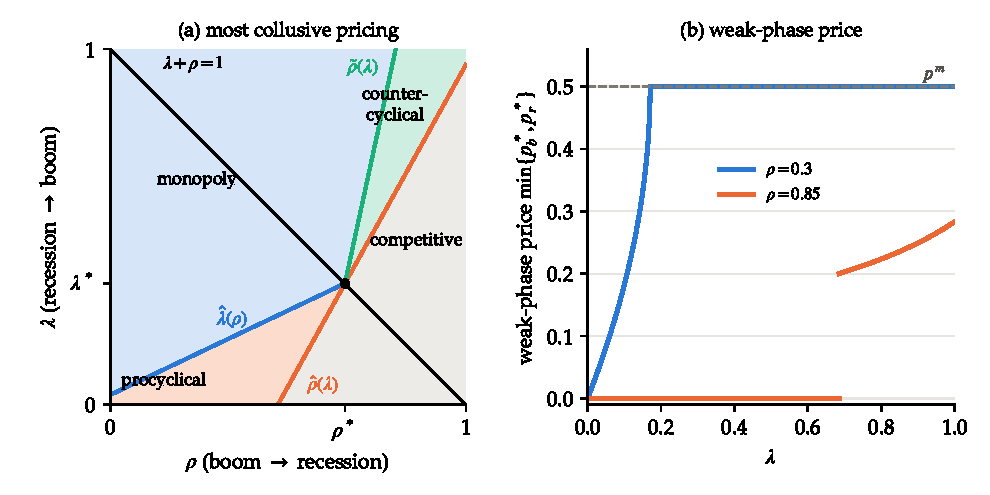
\includegraphics[width=\textwidth]{figures/ch12/bs_regions.pdf}
\caption{Most collusive pricing in the Markov-growth game for $N = 2$, $\delta = 0.9$, $g_b = 1.05$, $g_r = 0.30$,
$\pi(p) = p(1-p)$, $c = 0$. Panel (a): regions in the space of transition probabilities $(\rho, \lambda)$. Below the
anti-diagonal growth rates are positively correlated, above it negatively. The boundaries $\hat\lambda(\rho)$,
$\hat\rho(\lambda)$ and $\tilde\rho(\lambda)$ are \eqref{eq:12-bs-boundaries}, and they meet at $(\rho^*, \lambda^*) \approx (0.659, 0.341)$.
Panel (b): the price in the weak phase as a function of $\lambda$. For $\rho = 0.3$ pricing is procyclical for $\lambda < 0.17$, and
the recession price rises toward $p^m$ as recessions become shorter. For $\rho = 0.85$ pricing is competitive for
$\lambda < 0.686$, then countercyclical with a jump at the boundary. This redraws, with computed regions, Figure 1 of
\citet{BagwellStaiger1995}. Script \texttt{bs\_regions.py}.}
\label{fig:12-bs-regions}
\end{figure}

\subsubsection{Shocks within phases}

The basic model has deterministic demand within a phase. Section V of the paper adds random shocks within phases and
brackets the possibilities with two extremes (WP pp.~24--33). Firms observe the current shock before setting prices.

\casehead{Permanent shocks}
Let $G_t = g_t G_{t-1}\eta_t$, where $\eta_t$ is a multiplicative shock with mean one that becomes part of the base for
all future growth. (Bagwell and Staiger write $\epsilon_t$.) The most
collusive prices depend on the phase but not on the shock. The future is proportional to $G_t$, which already
includes $\eta_t$, so the shock cancels from the incentive constraints, as $G_t$ did before. Formally, the constraints
(WP (22)--(25)) reduce to \eqref{eq:12-bs-ic-b}--\eqref{eq:12-bs-W-r} once $G_t$ is cancelled and $\E[\eta_{t+1}] = 1$ is imposed.
Pricing is exactly as in the basic model (WP Theorem 5).

\casehead{Transitory shocks}
Let $G_t = g_t\frac{G_{t-1}}{\eta_{t-1}}\eta_t$, with $\eta_t$ independent over time, mean one and support $[\underline\eta, \bar\eta]$
containing one. The base level grows without the shock, and the shock affects only the current period. This combines
the Markov phases with Rotemberg-Saloner shocks. Let $p_b(\eta)$ and $p_r(\eta)$ be the prices in each phase when
the current shock is $\eta$. The base level cancels again, but the current shock does not. The boom constraint becomes
(WP (26))
\begin{equation*}
\eta\,\Gamma(p_b(\eta)) \le \delta\left[\rho g_r W_r + (1-\rho)g_b W_b\right],
\end{equation*}
with $W_b$ and $W_r$ defined as before but with $\E[w(p(\eta))\eta]$ in place of $w(p)$ (WP (28)--(29)). The paper solves
the system in two steps, following Rotemberg and Saloner. First it holds the right sides fixed at values
$\tilde W_b$ and $\tilde W_r$. Each constraint then reads $\pi(p_s(\eta)) \le \frac{N}{N-1}\frac{\tilde W_s}{\eta}$ (WP (34)--(35)), and the most
collusive price is
\begin{equation}\label{eq:12-bs-transitory-price}
p_s(\eta) = P^*\!\left(\frac{\tilde W_s}{\eta}\right) \equiv
\begin{cases}
p^m & \text{if } \pi(p^m) \le \frac{N}{N-1}\frac{\tilde W_s}{\eta},\\
\min\left\{p : \pi(p) = \frac{N}{N-1}\frac{\tilde W_s}{\eta}\right\} & \text{otherwise}
\end{cases}
\end{equation}
(WP (36)--(39)). Second, it requires the values $\tilde W_b$ and $\tilde W_r$ to be consistent with the prices they generate
(WP (40)--(43)). It then picks the largest fixed point of the resulting pair of equations. The competitive outcome
$\tilde W_b = \tilde W_r = 0$ is always a fixed point. To leave room for perfect collusion the paper assumes (WP (44))
\begin{equation*}
\delta g_b > \frac{\bar\eta(N-1)}{1 + \bar\eta(N-1)},
\end{equation*}
which says that even the largest shock would not disrupt perfect collusion if growth stayed at the boom rate forever.
To check this, apply the argument of \cref{prop:12-bs-stationary} with current demand scaled by $\bar\eta$:
$\bar\eta(N-1) \le \frac{\delta g_b}{1 - \delta g_b}$ rearranges to the displayed condition.

The results are Theorem 6 of the working paper. Both phases use the same pricing function $P^*$ in
\eqref{eq:12-bs-transitory-price}, and $P^*$ is nondecreasing in $\frac{\tilde W}{\eta}$. So a higher transitory shock lowers the
most collusive price weakly, in booms and in recessions alike. This is the Rotemberg-Saloner effect, now inside each
phase. The comparison between phases still follows the correlation of growth rates. Under positive correlation the
boom value exceeds the recession value at the most collusive fixed point, so $p_b(\eta) \ge p_r(\eta)$ at every shock,
with strict inequality for large shocks. Negative correlation reverses the ranking. The paper's Figures 6a and 6b show
both price schedules flat at $p^m$ for small shocks and falling for large ones. The boom schedule lies above the
recession schedule under positive correlation and below it under negative correlation. Transitory shocks also enlarge
the parameter region with cyclical pricing, because perfect collusion in both phases and at every shock now requires
more. The paper concludes that its second point ``provides an interpretation of the Rotemberg-Saloner (1986) theory in
terms of the transitory demand shocks that occur within broader business-cycle phases'' (WP p.~33).

\subsubsection{Empirical content and limits}

The theory makes the cyclicality of collusive prices an empirical question about the demand process of each industry.
The direction of the cycle depends on the correlation of growth rates, and its amplitude on the expected durations of
booms and recessions. Bagwell and Staiger suggest estimating these parameters industry by industry with Hamilton's
methods and comparing the predictions with industry prices (WP p.~34). No such study existed when they wrote. For
the aggregate economy, \citet{Hamilton1989} finds that quarterly growth rates of U.S. real GNP are positively correlated
and that booms last longer in expectation than recessions. If an industry's demand cycle shares these features, the
prediction of procyclical collusive prices ``appears most salient'' (WP p.~34). Existing evidence points both ways,
and the paper calls it mixed and inconclusive (WP p.~2 and fn.~4). It cites cross-industry studies of margins
\citep{DomowitzHubbardPetersen1986,RotembergWoodford1992}. It cites industry studies, among them
\citet{BorensteinShepard1996}, \citet{Ellison1994}, \citet{Porter1983} and \citet{RotembergSaloner1986}. It also cites
evidence that cartels are most likely to break down during recessions \citep{Suslow1988}.

The authors list three limits (WP pp.~34--35). Marginal costs are acyclic in the model, while the evidence on their
cyclicality is mixed \citep{Bils1987,MironZeldes1988}. Firms are assumed to tell transitory shocks from turning points.
If they observe only demand, they must infer the phase, and the sharp distinction between the responses to the two
kinds of movement will soften. Finally, the analysis is partial equilibrium. With entry and exit the difference between
phases may matter less, and with endogenous interest rates discounting may be more severe in booms.

\subsection{Comparing the models}\label{sec:12-demand-compare}

\Cref{tab:12-cycle-theories} compares the theories of this section with the imperfect-monitoring theory of the next.
The models agree on the logic of the incentive constraint. They disagree on what current demand reveals about the
future and on what firms observe. These two features decide when collusive prices are lowest and whether price wars
appear on the equilibrium path. The table also suggests what data would tell the theories apart. One needs the timing
of low prices relative to the level, growth and predictability of demand. One also needs to know whether low prices
follow observed or unobserved shocks. \Cref{ch:collusion-evidence} takes these predictions to the data.

\begin{table}[htbp]
\centering
\caption{Demand fluctuations and collusive pricing: four theories compared}\label{tab:12-cycle-theories}
\footnotesize
\begin{tabularx}{\textwidth}{@{}>{\raggedright\arraybackslash}p{2.35cm}>{\raggedright\arraybackslash}X>{\raggedright\arraybackslash}X>{\raggedright\arraybackslash}p{2.2cm}>{\raggedright\arraybackslash}X@{}}
\toprule
Model & What drives the future loss & When collusive prices are lowest & Price wars on the path? & Testable implication\\
\midrule
\citet{RotembergSaloner1986}: observed independent shocks & Expected demand, the same in every state & In high-demand states, above a cutoff & No (yes only with collude-or-compete strategies) & Margins fall when current demand is high\\[3pt]
\citet{HaltiwangerHarrington1991}: deterministic cycle & Demand along the known future path & When demand is about to fall, and at the peak for impatient firms & No & At equal demand, prices higher when demand rises than when it falls\\[3pt]
\citet{BagwellStaiger1997}: Markov growth phases & Expected future growth, which depends on the phase & In recessions under positive correlation, in booms under negative correlation & No & Direction and amplitude of the price cycle depend on correlation and phase durations\\[3pt]
\citet{GreenPorter1984}: unobserved shocks (\cref{sec:12-public}) & Probability that a low price triggers a war & After unexpectedly low demand & Yes, finite reversions & Wars follow negative demand shocks and are not caused by cheating\\
\bottomrule
\end{tabularx}
\end{table}
